\documentclass[letterpaper, 11pt]{article}
\usepackage{comment} % enables the use of multi-line comments (\ifx \fi) 
\usepackage{fullpage} % changes the margin
\usepackage{fancyhdr} % for footerhttps://www.overleaf.com/3039851kkndbp#
\usepackage[UKenglish]{isodate}% http://ctan.org/pkg/isodate for date format
\usepackage{float}%force tables/figs into certain placement
\usepackage{changepage}%for dichotomous key
\usepackage{graphicx}%for figures
\usepackage{caption}%for figures
\usepackage{subcaption}%for figures
\usepackage{hyperref}
\usepackage{textcomp}
\usepackage{natbib}
\usepackage{placeins}%prevent images from floating into inappropriate sections

\newcommand*{\doi}[1]{\href{http://dx.doi.org/#1}{doi: #1}}% links DOI
\usepackage{epigrafica}%changes default font to epigrafica
\DeclareTextAccent{\"}{OT1}{168}%declare umlaut
\usepackage{placeins}%prevent images from floating into inappropriate sections
\newcommand{\latinword}[1]{\texttt{\itshape #1}}%use \latinword for vocab
\def\labelitemi{--} %change bullet to em dash
\pagestyle{fancy}
\renewcommand{\headrulewidth}{0pt}

\lhead{}
\chead{}
\rhead{}
\lfoot{ENT 432 (Fall 2016) - Penn State}
\cfoot{}
\rfoot{\thepage}
\renewcommand{\footrulewidth}{0.4pt}
\title{Unit 7 - Paleoptera, Plecoptera, origin of wings}
\author{Open Entomology Project}

\begin{document}
\cleanlookdateon %removed ordinal date
\maketitle
\thispagestyle{fancy}
\section*{Introduction}
In the insect phylogeny and fossil record we observe several adaptive radiations---\textit{i.e.}, events where the emergence of some key innovation (or opportunity) facilitates the rapid diversification of new forms. The emergence of wings is arguably the most important of these key innovations, yet the origin of the structures and the selective forces that acted on early versions of wings remain enigmatic. We will discuss hypotheses of the origin of wings, including the strength of their evidence, before moving on to \textbf{Paleoptera} (or Palaeoptera) and the neopteran order \textbf{Plecoptera}.

\section*{Materials}

\begin{itemize}
\item specimens (provided)
\item fine forceps, probes (provided)
\item sorting tray, watch glasses, gloves, safety glasses, glycerine, ethanol (provided)
\item pencil/paper for sketches
\end{itemize}

\section*{Safety}
We will be working with sharp tools. Wear your personal protective gear at all times. Specimens are to be returned to their vials after lab, and glycerine and ethanol will be collected for proper disposal or reuse.

\section*{Methods}
Working with a partner, organize your space, specimens, tools, and microscope. Use your probe and forceps to manipulate the specimen. In this lab, however, we will not be dissecting specimens (unless otherwise noted). You can start anywhere in the handout.

\section*{Insecta: Pterygota}
We're now looking at insects that have \textit{wings}, which are usually present as two pairs: fore wings, which articulate with the mesothorax, and hind wings, which articulate with the metathorax.\\

\hangindent2em\textbf{Question 7-1:} Why is the thoracic integument so heavily sclerotized, relative to other body parts and those structures in non-pterygote hexapods? What are the consequences of this phenotype?\\

\hangindent2em\textbf{Question 7-2:} Why aren't there wings on the prothorax?

\section*{Pterygota: Palaeoptera}
In the next two orders, the wing base inhibits wing folding (\textit{i.e.}, wings held out or vertically over the thorax when at rest). The latest evidence indicates that these two orders comprise a monophyletic group, called Palaeoptera.

\section{Ephemeroptera (mayflies)}

\subsection{Naiads}
Mayflies are aquatic as immatures, and these stages are usually referred to as naiads or larvae (Not to be confused with the immature stages of holometabolous insects; more on that later.) Mayflies also spend the vast majority of their lives as naiads, and we can observe numerous adaptations for feeding and locomotion. We have naiads of the following three families, which should give you a sense of the phenotypic variation in Ephemeroptera: Baetidae, Hetageniidae, and Ephemeridae. After observing the immature stages see if you can answer the following questions:\\

\hangindent2em\textbf{Question 7-3:} The bodies and head shapes of these mayflies yield clues about their life histories. Can you predict where each family is typically found and how eat it eats and moves through the water?\\

\hangindent2em\textbf{Question 7-4:} Can you find evidence of developing wings or even evidence that suggests the origin of wings?\\

\begin{figure}[ht!]
  \centering
    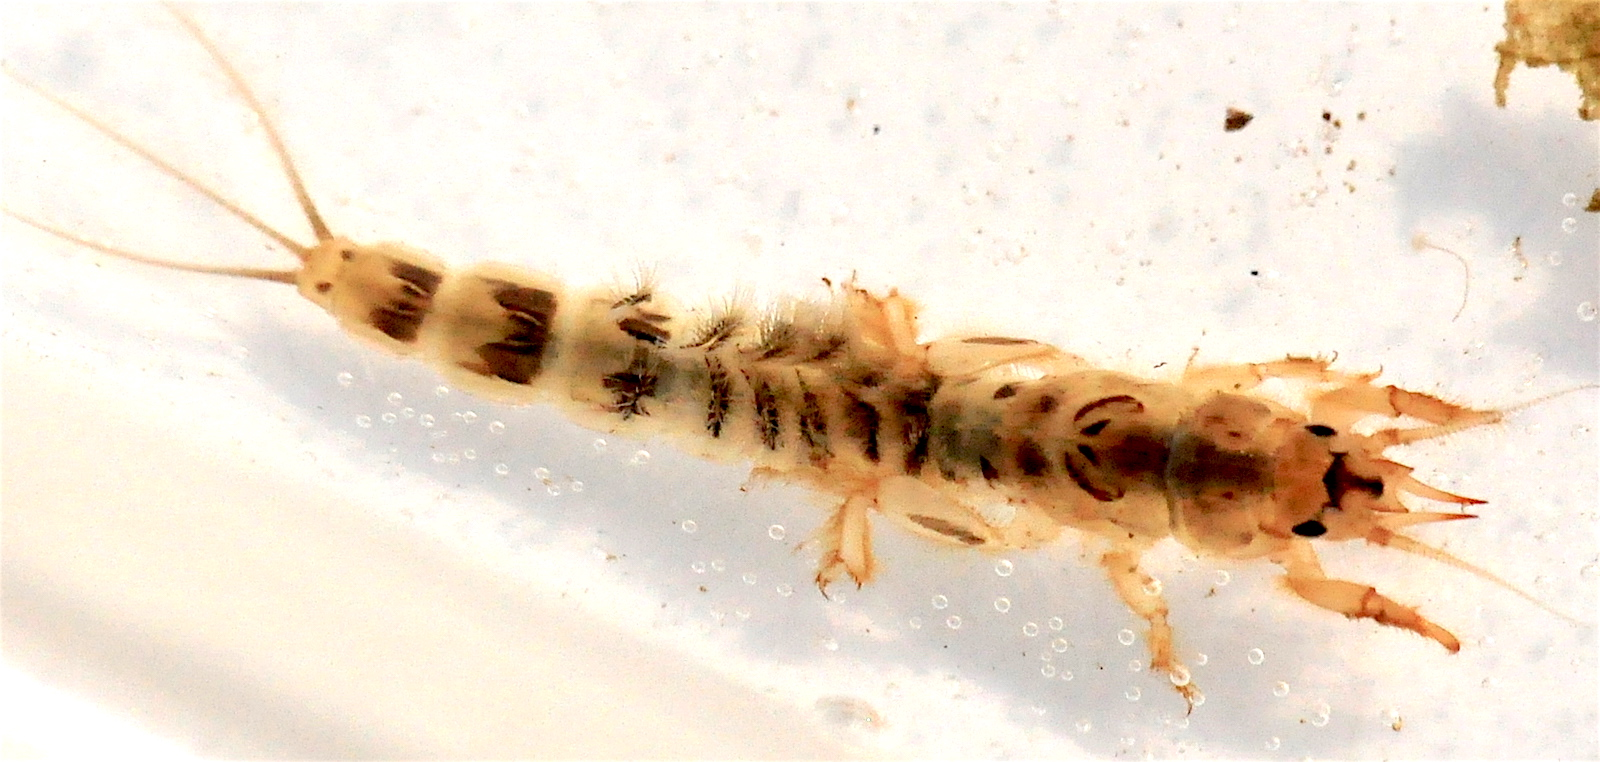
\includegraphics[width=0.45\textwidth]{EphemeridLarva}
  \caption{Ephemeridae larva. Photo (CC BY-NC 2.0) by Roger Sanderson \url{https://flic.kr/p/fEVW7i}}
  \label{fig:ephemeridlarva}
\end{figure}

\begin{figure}[ht!]
    \centering
    \begin{subfigure}[ht!]{0.47\textwidth}
        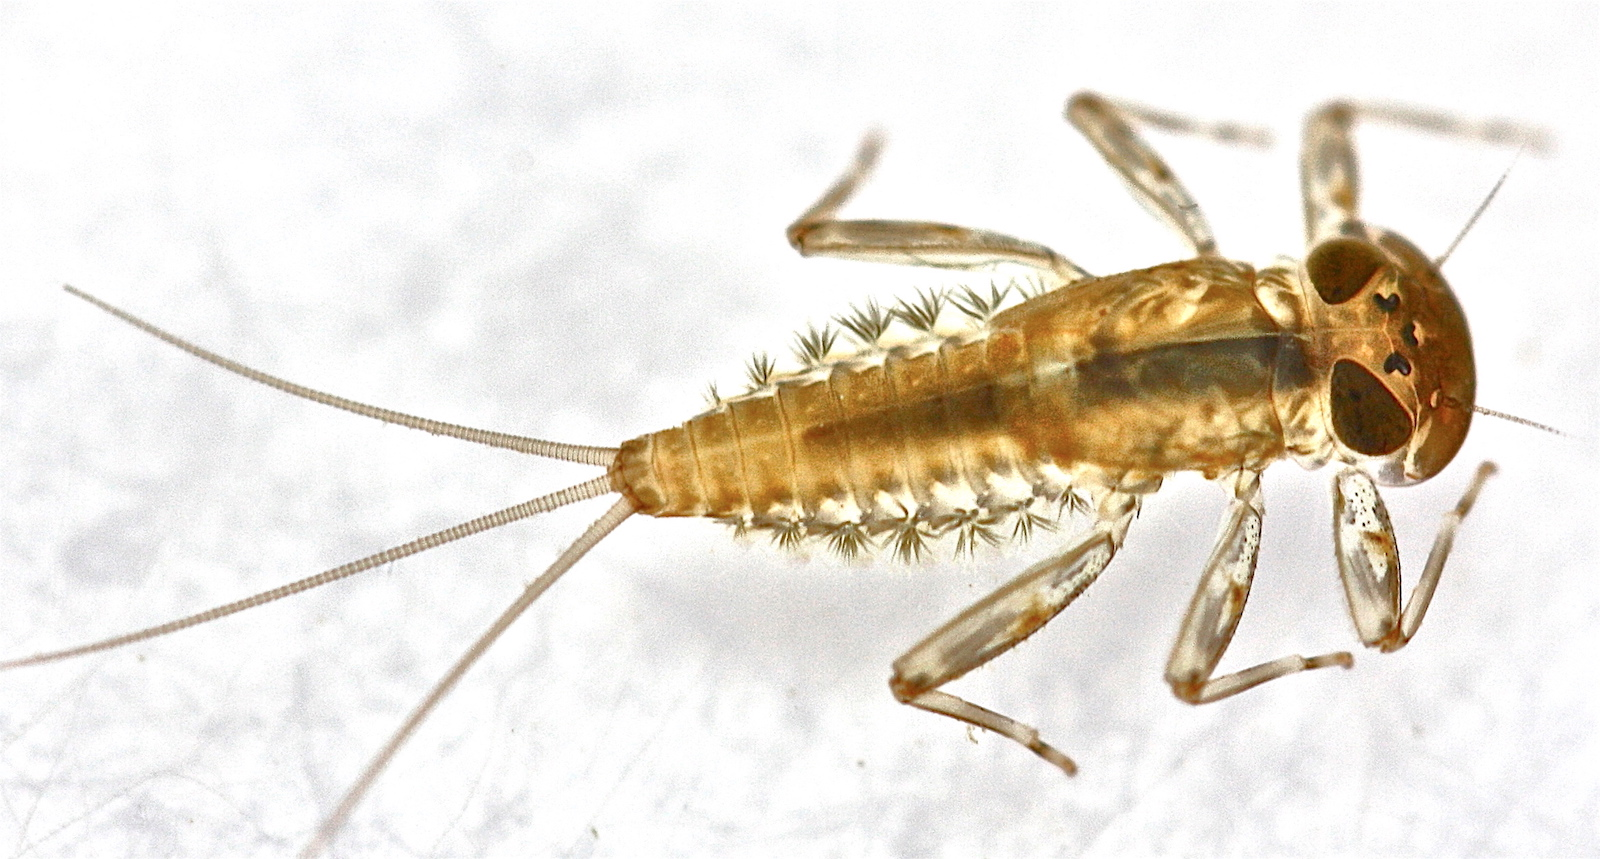
\includegraphics[width=\textwidth]{HeptageniidLarva}
        \caption{Heptageniidae larva. Photo (CC BY-NC 2.0) by Bob Henricks \url{https://flic.kr/p/9ExxWu}}
        \label{fig:heptageniidlarva}
    \end{subfigure}
    \hfill
    \begin{subfigure}[ht!]{0.46\textwidth}
        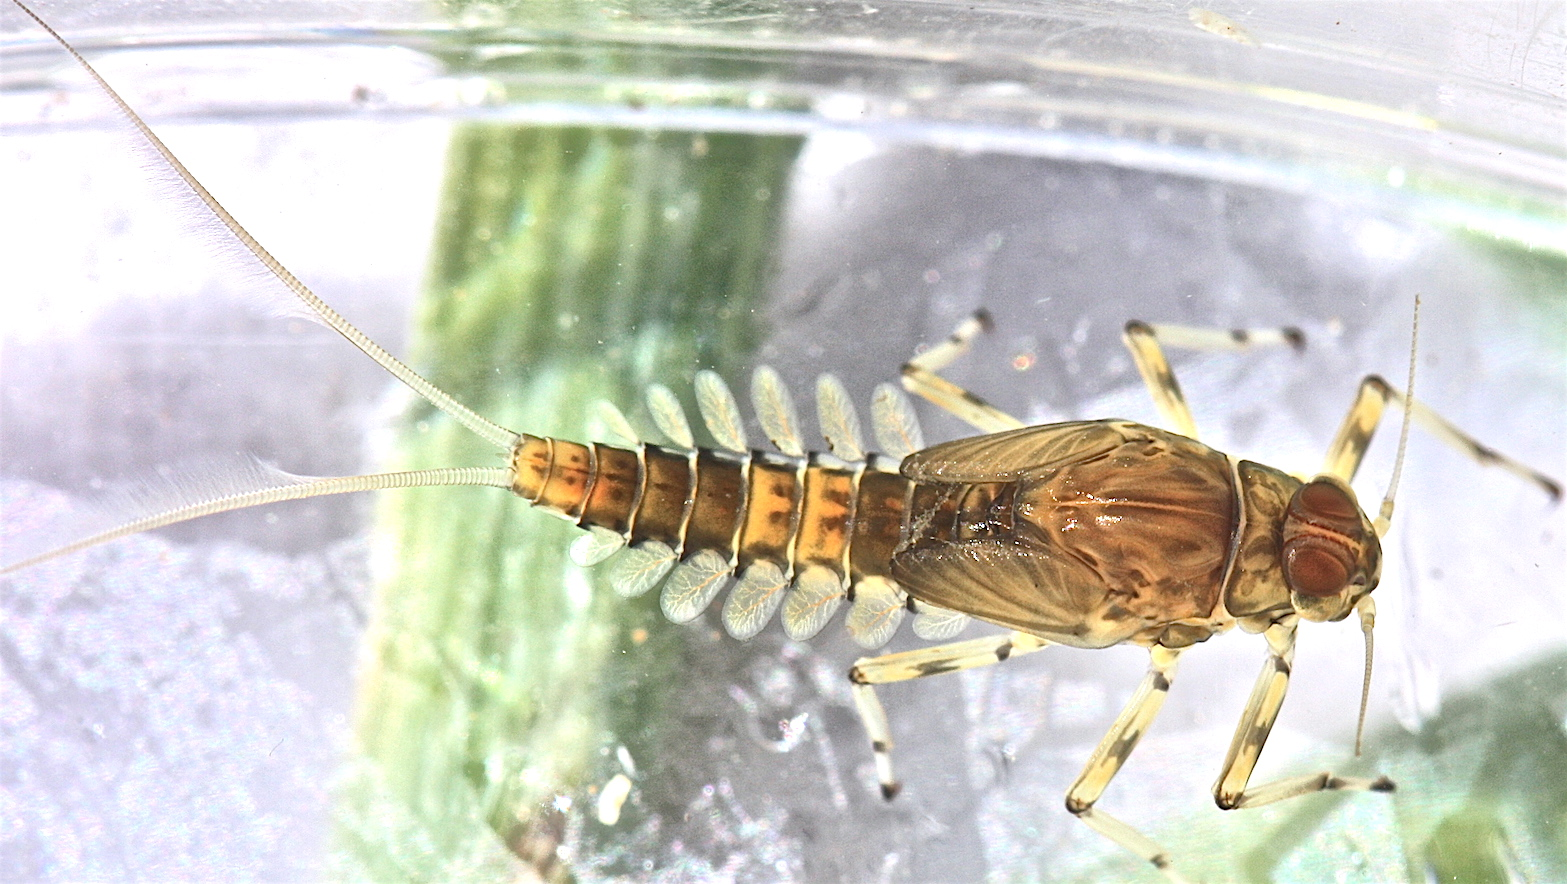
\includegraphics[width=\textwidth]{BaetidLarva}
        \caption{Baetidae habitus. Photo (CC BY-NC 2.0) by Bob Henricks \url{https://flic.kr/p/bqgXsZ}}
        \label{fig:baetidlarva}
    \end{subfigure}
    \label{fig:mayflylarvae}
\end{figure}
\FloatBarrier

\subsection{Adults}
\noindent{}Wing venation and appendage phenotype offer important characters for family-level diagnosis of adults. See if you can understand the following set of characters, which could be used to recognize adults of three common families in Pennsylvania: Ephemeridae, Heptageniidae, and Baetidae. Note that these are not the only families you can collect easily!

\begin{itemize}
\item Male compound eye morphology: 0 = round, unmodified (Ephemeridae, Heptageniidae), 1 = turbinate (Fig. \ref{fig:baetid2}) (Baetidae)
\item Cubital intercalaries (between CuA and CuP) in fore wing: 0 = present as 2 parallel pairs (Heptageniidae), 1 = not present as 2 parallel pairs (Baetidae, Ephemeridae)
\item Angle of \texorpdfstring{MP\textsubscript{2}}{ }{ }of fore wing: 0 = sharply angled towards Cu proximally (Ephemeridae), 1 = not sharply angled towards Cu proximally (Baetidae, Heptageniidae)
\item Hind wing relative size: 0 = Very small, in some species almost absent (Baetidae), 1 = large, visible, with many veins (Ephemeridae, Heptageniidae)
\item Hind leg tarsus subdivision number: 0 = 5 tarsomeres (Heptageniidae), 1 = 4 tarsomeres (Baetidae, some Ephemeridae), 2 = 3 tarsomeres (some Ephemeridae)
\item Apical appendage number (\textit{i.e.}, the thread-like appendages that are not genitalia): 0 = 3 (some Ephemeridae), 1 = 2 (\textit{i.e.}, the median filamentous appendage is absent) (Baetidae, Heptageniidae, some Ephemeridae)
\end{itemize}

\begin{figure}[ht!]
  \centering
    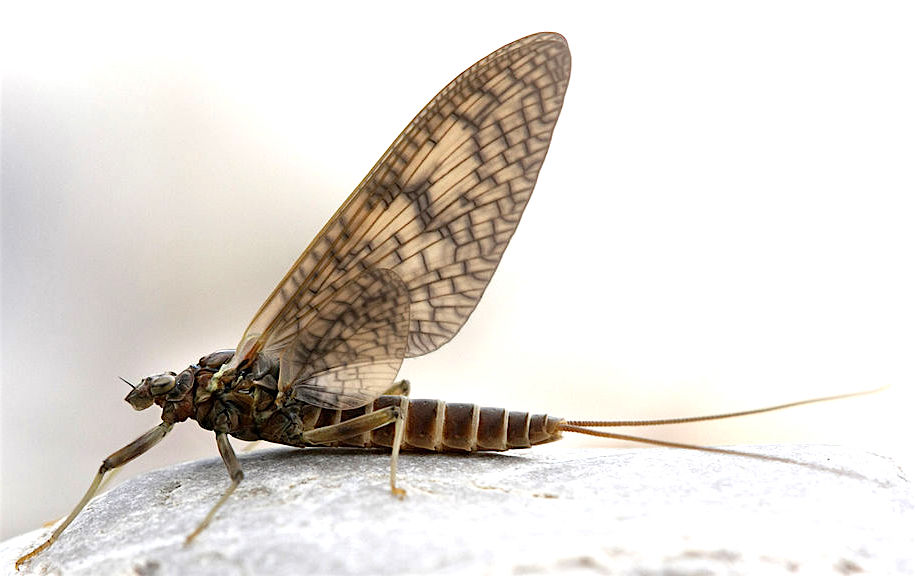
\includegraphics[width=0.5\textwidth]{HeptageniidHabitus}
  \caption{Heptageniidae. Photo (CC BY-SA 2.5) by Richard Bartz \url{https://goo.gl/lIU2qx}}
  \label{fig:heptageniid}
\end{figure}

\begin{figure}[ht!]
    \centering
    \begin{subfigure}[ht!]{0.35\textwidth}
        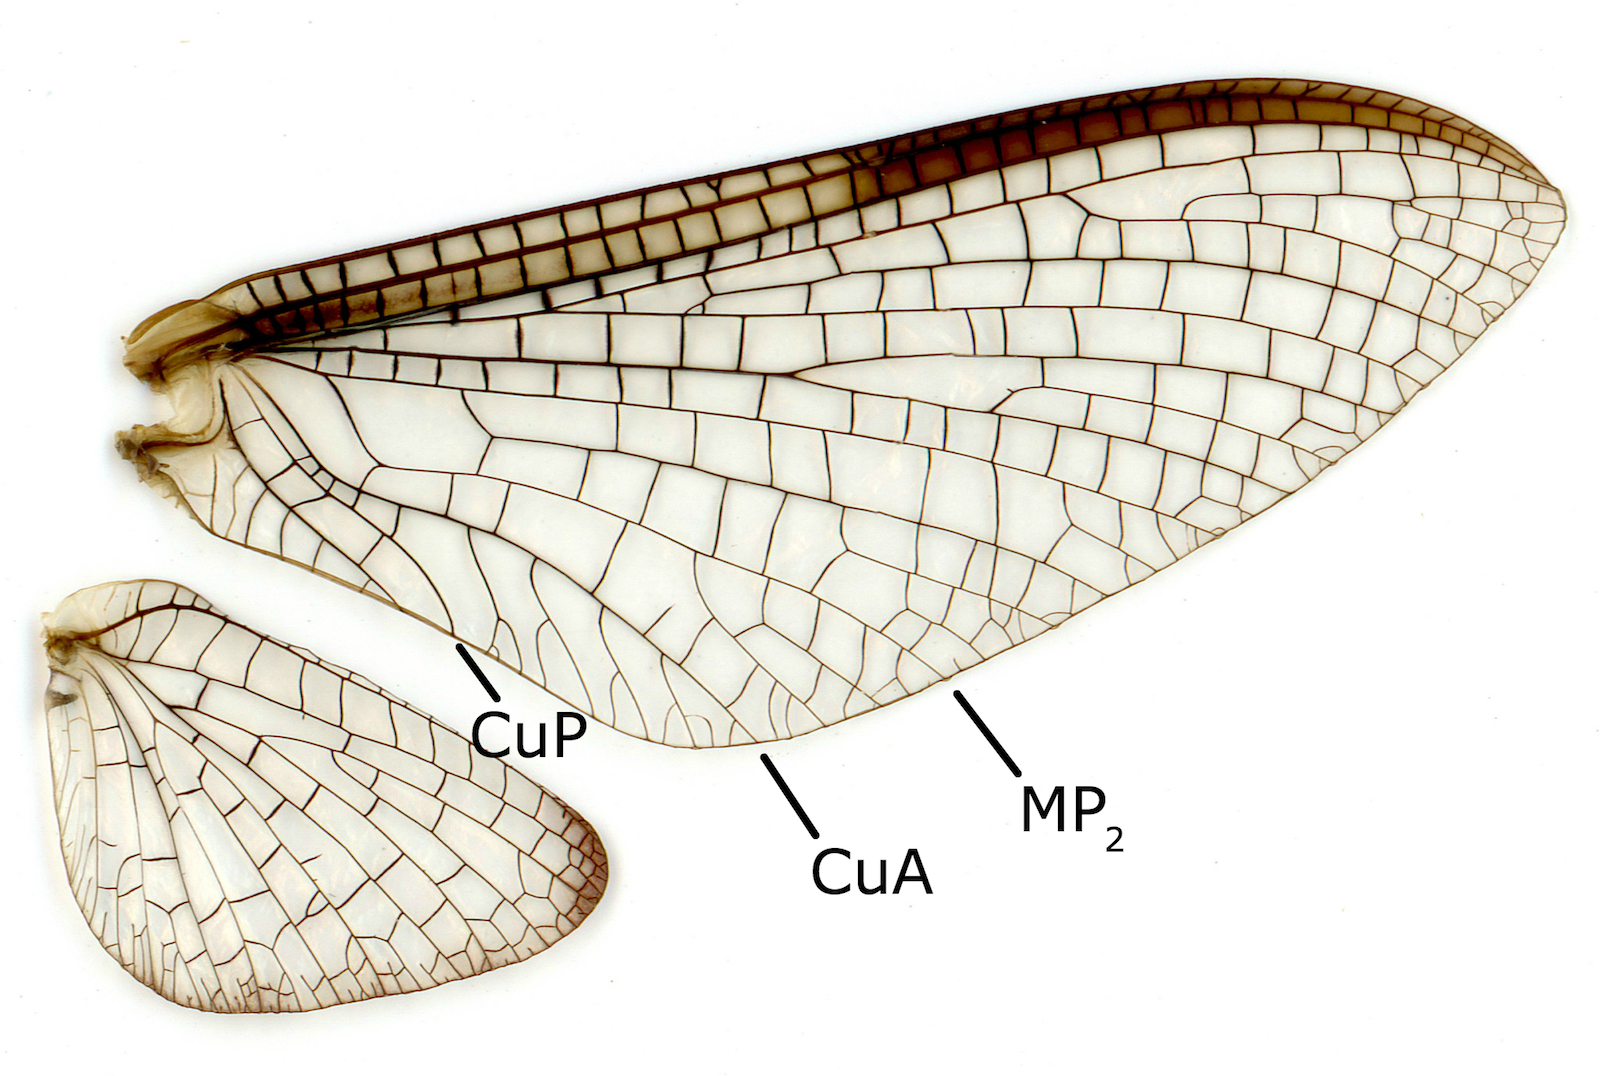
\includegraphics[width=\textwidth]{EphemeridWings}
        \caption{Wing venation. Photo (CC BY 2.0) by Andy Deans \url{https://flic.kr/p/nDpya5}}
        \label{fig:ephemwing}
    \end{subfigure}
    \hfill
    \begin{subfigure}[ht!]{0.60\textwidth}
        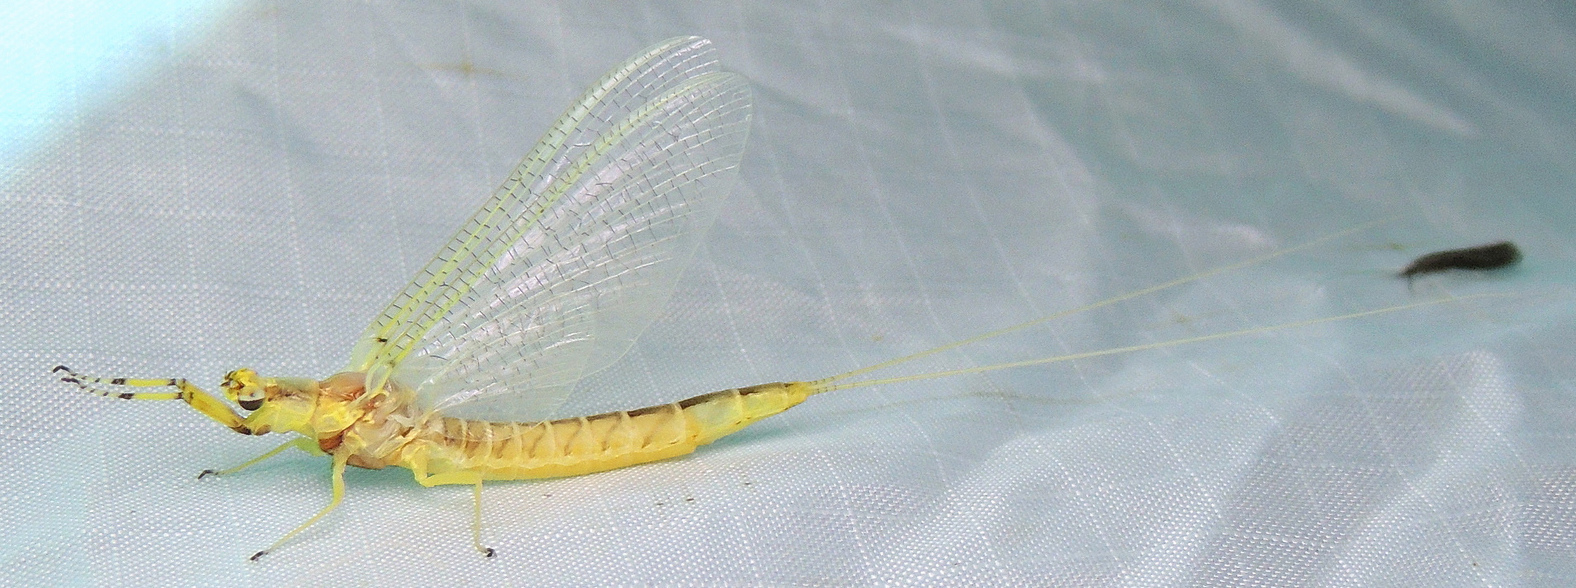
\includegraphics[width=\textwidth]{ephemeridbody}
        \caption{Habitus. Photo (CC BY-NC 2.0) by Anita Gould \url{https://flic.kr/p/f9eHPo}}
        \label{fig:ephemeridbody}
    \end{subfigure}
    \caption{Ephemeridae}\label{fig:ephemerid}
\end{figure}

\begin{figure}[ht!]
    \centering
    \begin{subfigure}[ht!]{0.45\textwidth}
        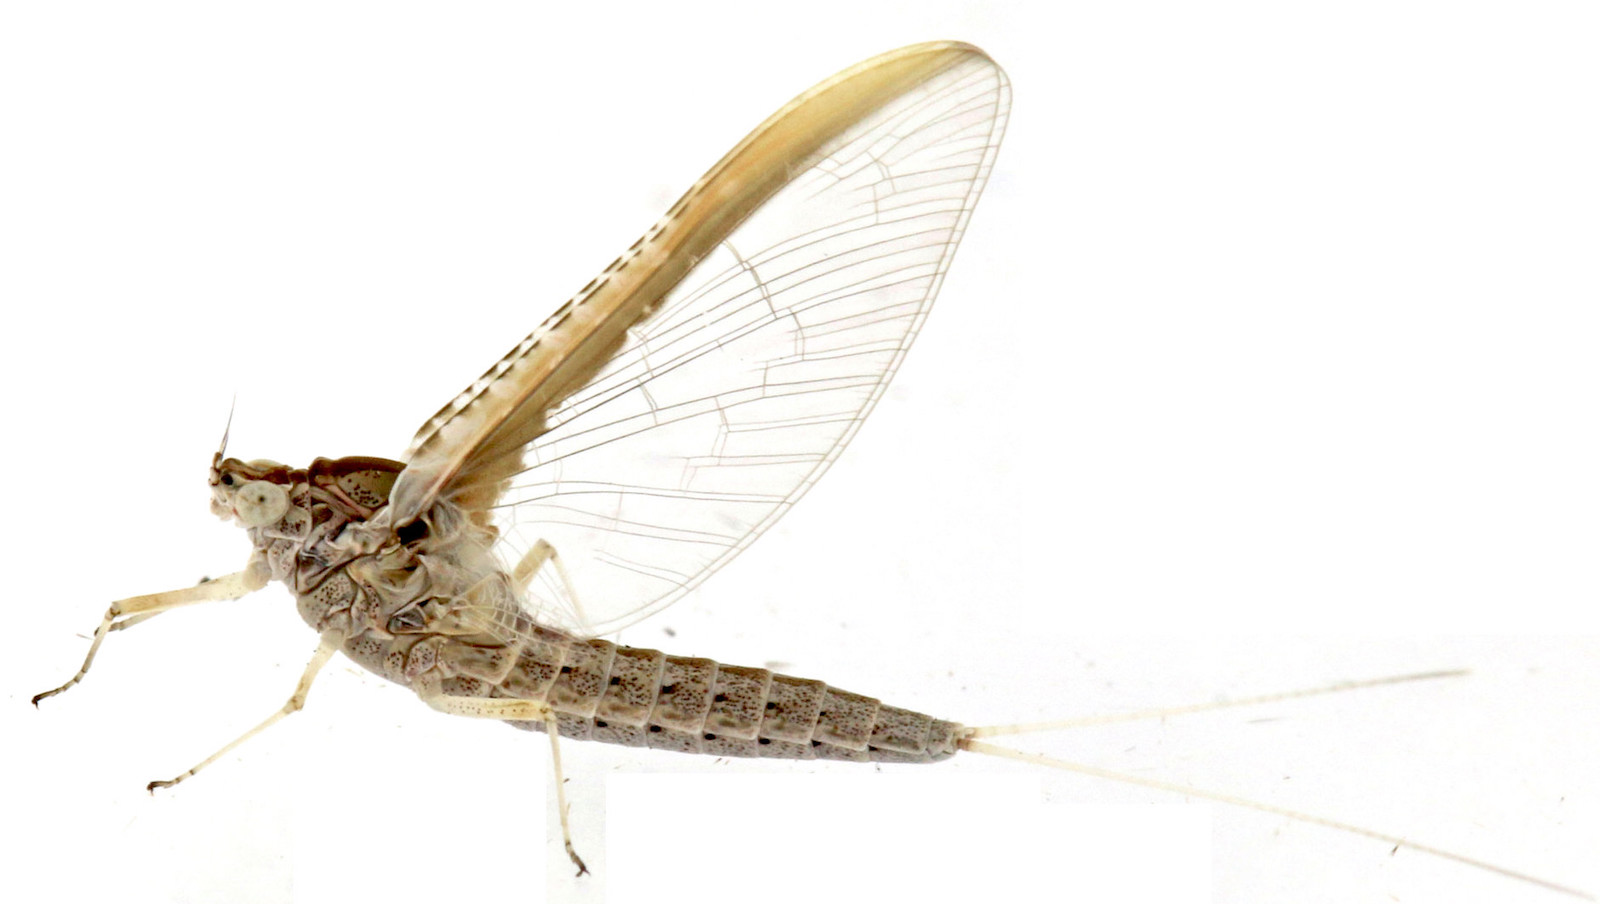
\includegraphics[width=\textwidth]{BaetidaeFemHabitus}
        \caption{Female habitus. Photo (CC BY 2.0) by Andrey Zharkikh \url{https://flic.kr/p/AnyRSm}}
        \label{fig:baetid1}
    \end{subfigure}
    \hfill
    \begin{subfigure}[ht!]{0.45\textwidth}
        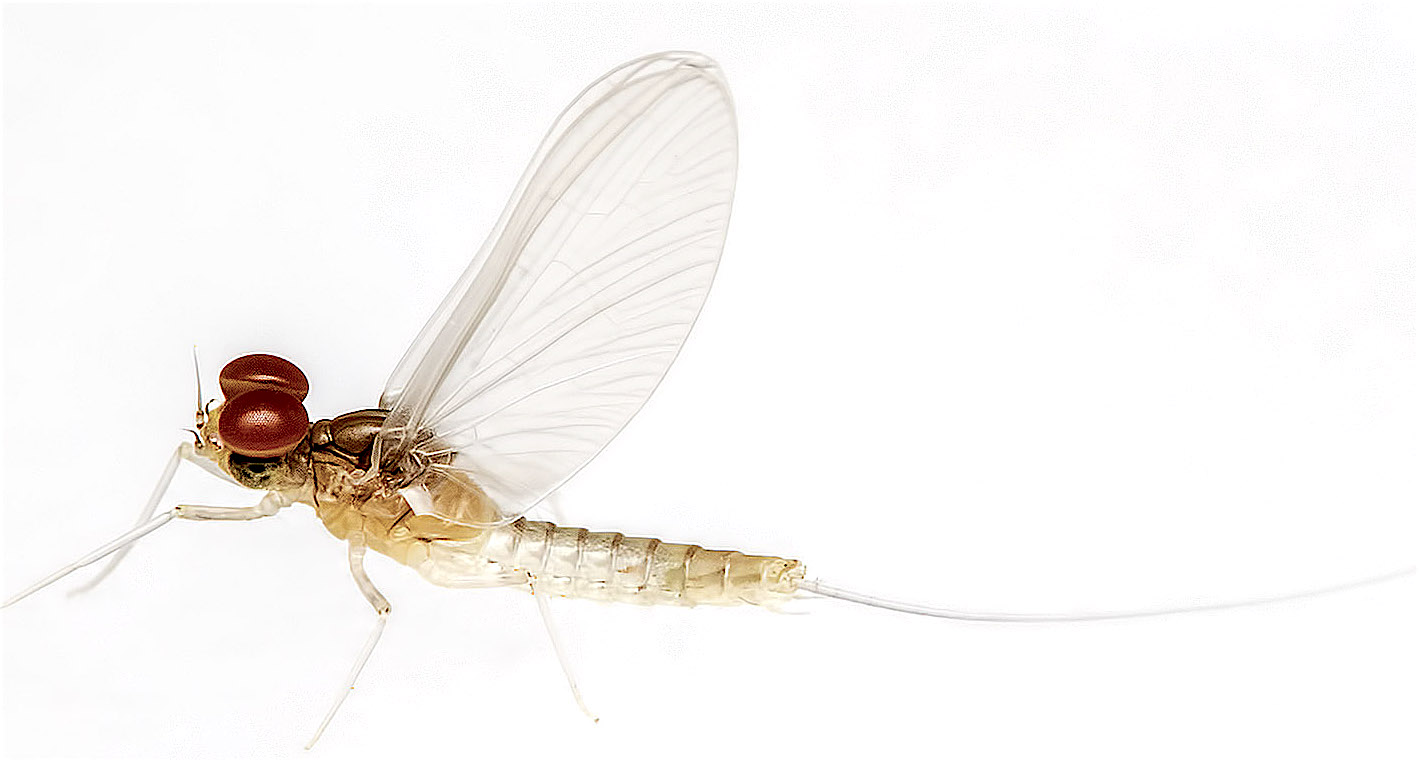
\includegraphics[width=\textwidth]{BaetidaeMaleHabitus}
        \caption{Male habitus, not conspecific with \ref{fig:baetid1}. Photo (CC BY 2.0) by A N Suresh Kumar \url{https://flic.kr/p/F3WMQQ}}
        \label{fig:baetid2}
    \end{subfigure}
    \caption{Baetidae}\label{fig:baetids}
\end{figure}

\FloatBarrier

\section{Odonata (dragonflies, damselflies)}%add larvae! crawlers, sprawlers, etc. look at adaptations
Like their putative sister lineage, immature Odonata are almost exclusively aquatic. All species are predaceous in all stages, with adaptations that facilitate prey tracking, stalking, and capture. \\

\hangindent2em\textbf{Question 7-5:} Can you list at least three adaptations you see across Odonata families that you hypothesize are adaptations for predation?\\

\noindent{}Another conspicuous synapomorphy for Odonata is the evolution of a secondary copulatory organ ventrally on the first abdominal segment of males. Females are grabbed and held behind the head by the male, using his apical abdominal appendages. Be sure to look for adaptations associated with this unusual copulatory habit.\\

\noindent{}Odonata is the first group where each wing has a distinct pterostigma (pigmented spot on anterior edge of wing). The pterostigma is not only highly pigmented but also more sclerotized and more massive than other wing areas. \\

\hangindent2em\textbf{Question 7-6:} What might be the function of the pterostigma in pterygote insects?\\

\subsection{Gomphidae (clubtails)}
\noindent{}\textit{Diagnostic characters:} Compound eyes separated dorsally, triangular wing cells (``triangles'') in fore wing and hind wing similar in shape and location, apical abdominal segments often expanded laterally.\\

\noindent{}\textit{Natural history:} Larvae are usually found in lotic systems, where they bury themselves in the substrate and wait for prey. Look for adults on flat perches, \textit{e.g.}, on the ground or on leaves. Approximately 900 spp. have been described worldwide.

\begin{figure}[ht!]
    \centering
    \begin{subfigure}[ht!]{0.5\textwidth}
        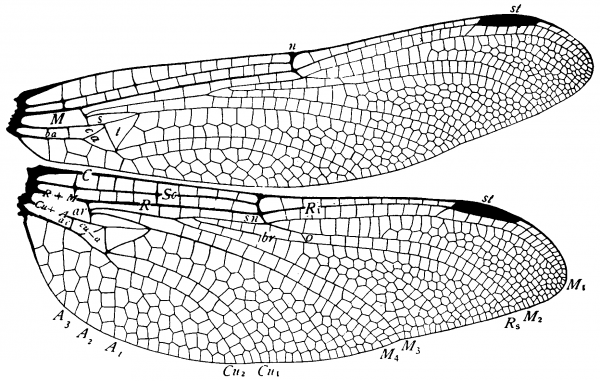
\includegraphics[width=\textwidth]{GomphidaeWing}
        \caption{Wing venation \citep[][Fig. 229]{comstock1918wings}}
        \label{fig:gomphid1}
    \end{subfigure}
    \hfill
    \begin{subfigure}[ht!]{0.4\textwidth}
        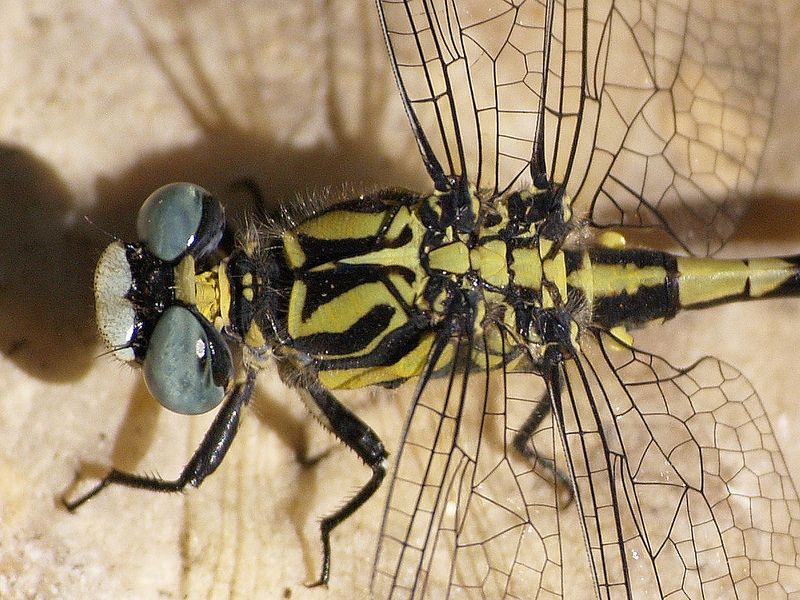
\includegraphics[width=\textwidth]{GomphidHead}
        \caption{Head and thorax. Photo (CC BY-NC-SA 2.0) by Matthew O’Donnell \url{https://flic.kr/p/dukePj}}
        \label{fig:gomphid2}
    \end{subfigure}
    \caption{Gomphidae}\label{fig:gomphids}
\end{figure}

\subsection{Aeshnidae (darners, hawkers)}
\noindent{}\textit{Diagnostic characters:} Compound eyes adjacent dorsally, triangular wing areas (``triangles'') in fore wing and hind wing similar in shape and location, ovipositor well developed.\\

\noindent{}\textit{Natural history:} Larvae are often thought of as being part of the ``climber'' guild of aquatic insects, as they are usually found in aquatic vegetation. Do they appear to be adapted for climbing and hunting in vegetation (see Fig. \ref{fig:OdonataLarva})? Adults are typically large and are very strong fliers. One can find these dragonflies in/near almost any aquatic habitat. Approximately 440 spp. have been described worldwide.\\

\begin{figure}[ht!]
    \centering
    \begin{subfigure}[ht!]{0.48\textwidth}
        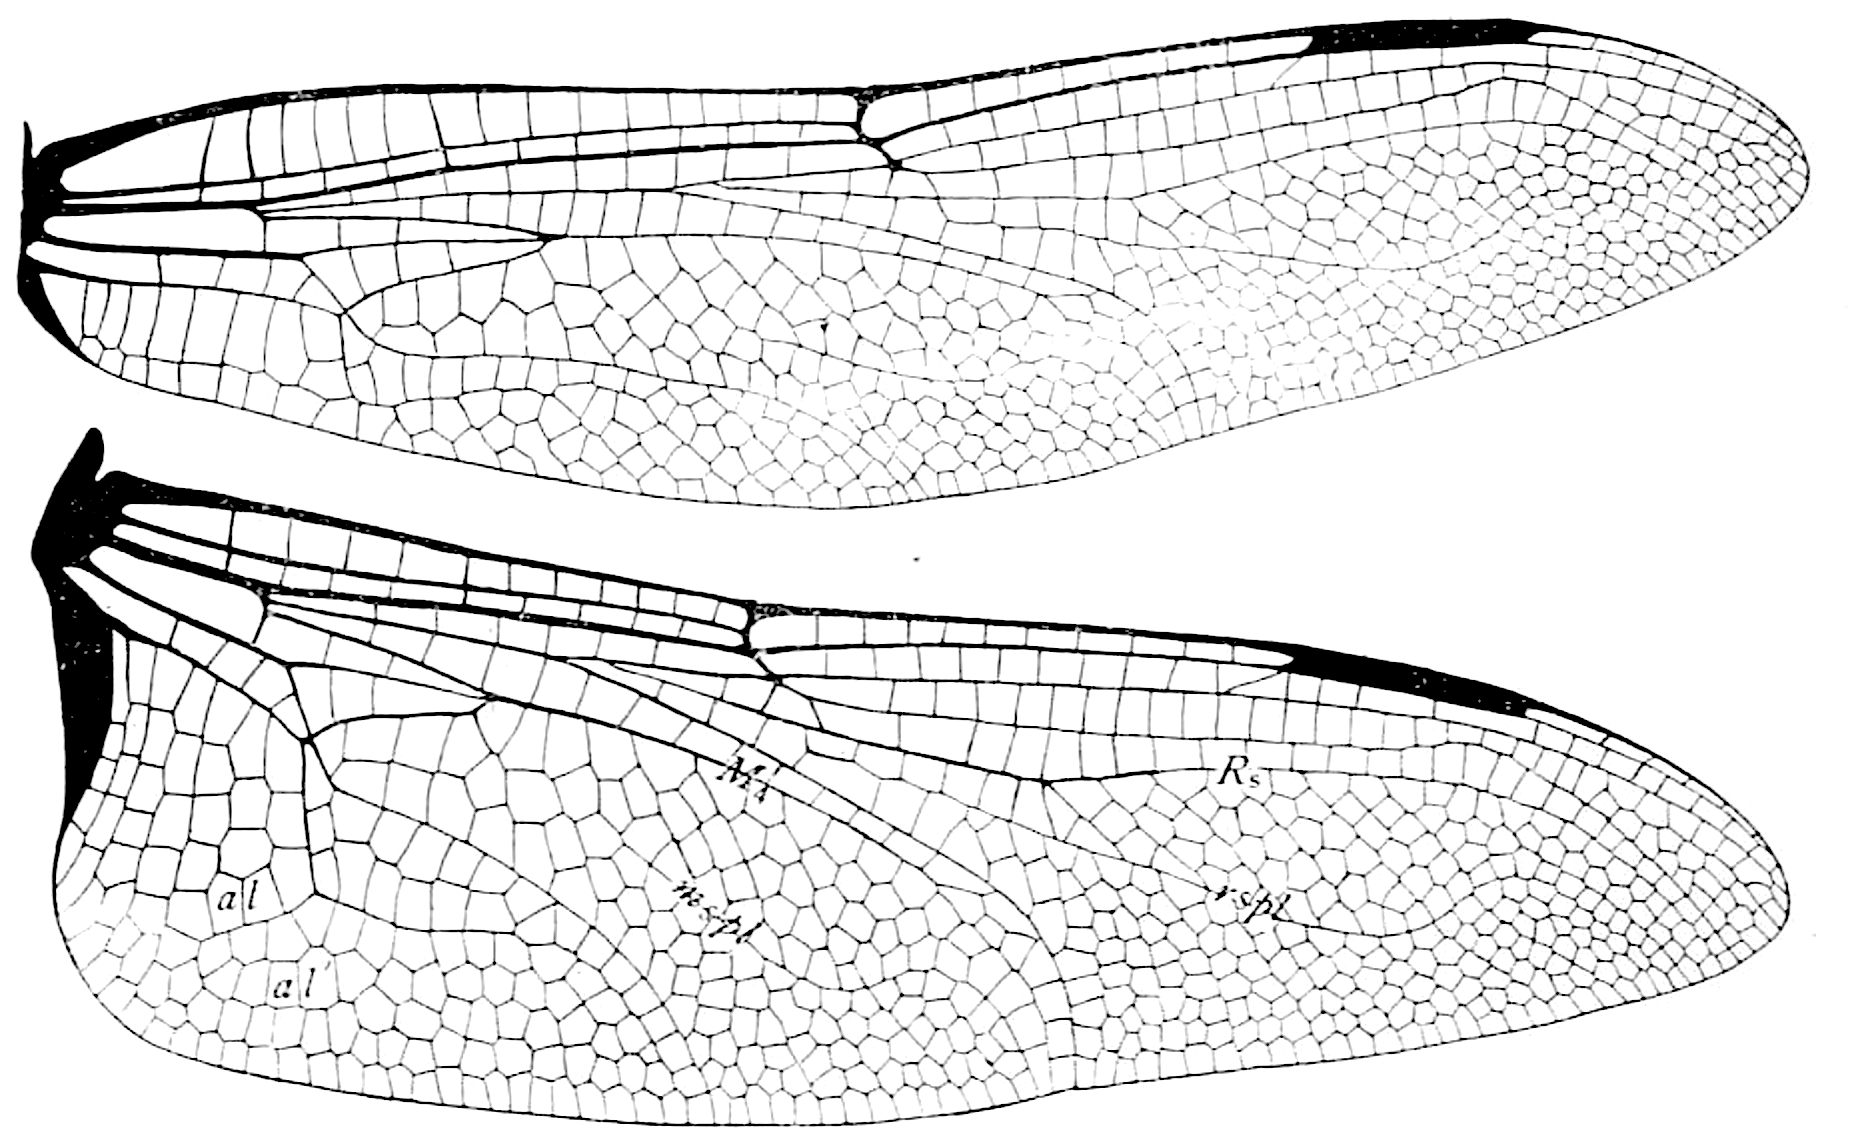
\includegraphics[width=\textwidth]{AeshnidWings}
        \caption{Wing venation \citep[][Fig. 236]{comstock1918wings}}
        \label{fig:aeshnid1}
    \end{subfigure}
    \hfill
    \begin{subfigure}[ht!]{0.42\textwidth}
        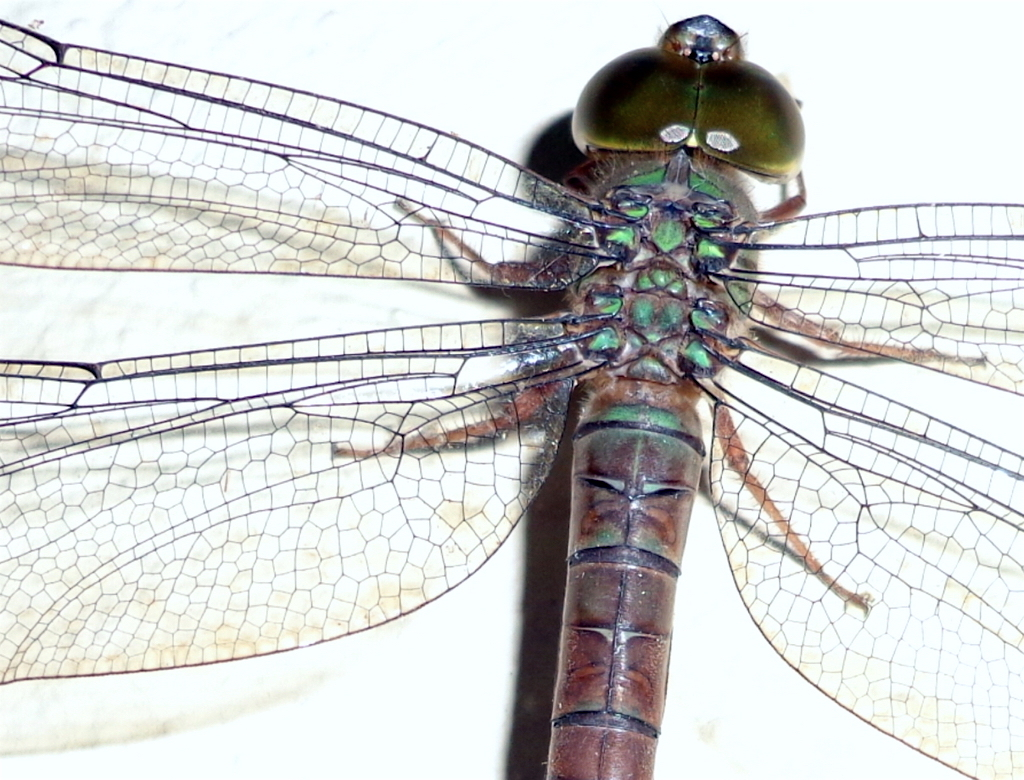
\includegraphics[width=\textwidth]{AeshnidHabitus}
        \caption{Habitus. Photo (CC BY-NC 2.0) by Adedotun Ajibade \url{https://flic.kr/p/fn8NtW}}
        \label{fig:aeshnid2}
    \end{subfigure}
    \caption{Aeshnidae}\label{fig:aeshnids}
\end{figure}

\subsection{Libellulidae (common skimmers)} 
\noindent{}\textit{Diagnostic characters:} Compound eyes meeting dorsally, triangles in fore wing and hind wing different in shape, hind wing with boot-shaped area, ovipositor absent.\\

\noindent{}\textit{Natural history:} Larvae are usually thought of as ``sprawlers'', which generally sit relatively still on the bottom, in the sediment, waiting for prey. Can you see major morphological differences between these larvae and other odonates? Adults are diverse in size, color, and habitat. More than 1,000 spp. have been described worldwide.\\

\begin{figure}[ht!]
    \centering
    \begin{subfigure}[ht!]{0.45\textwidth}
        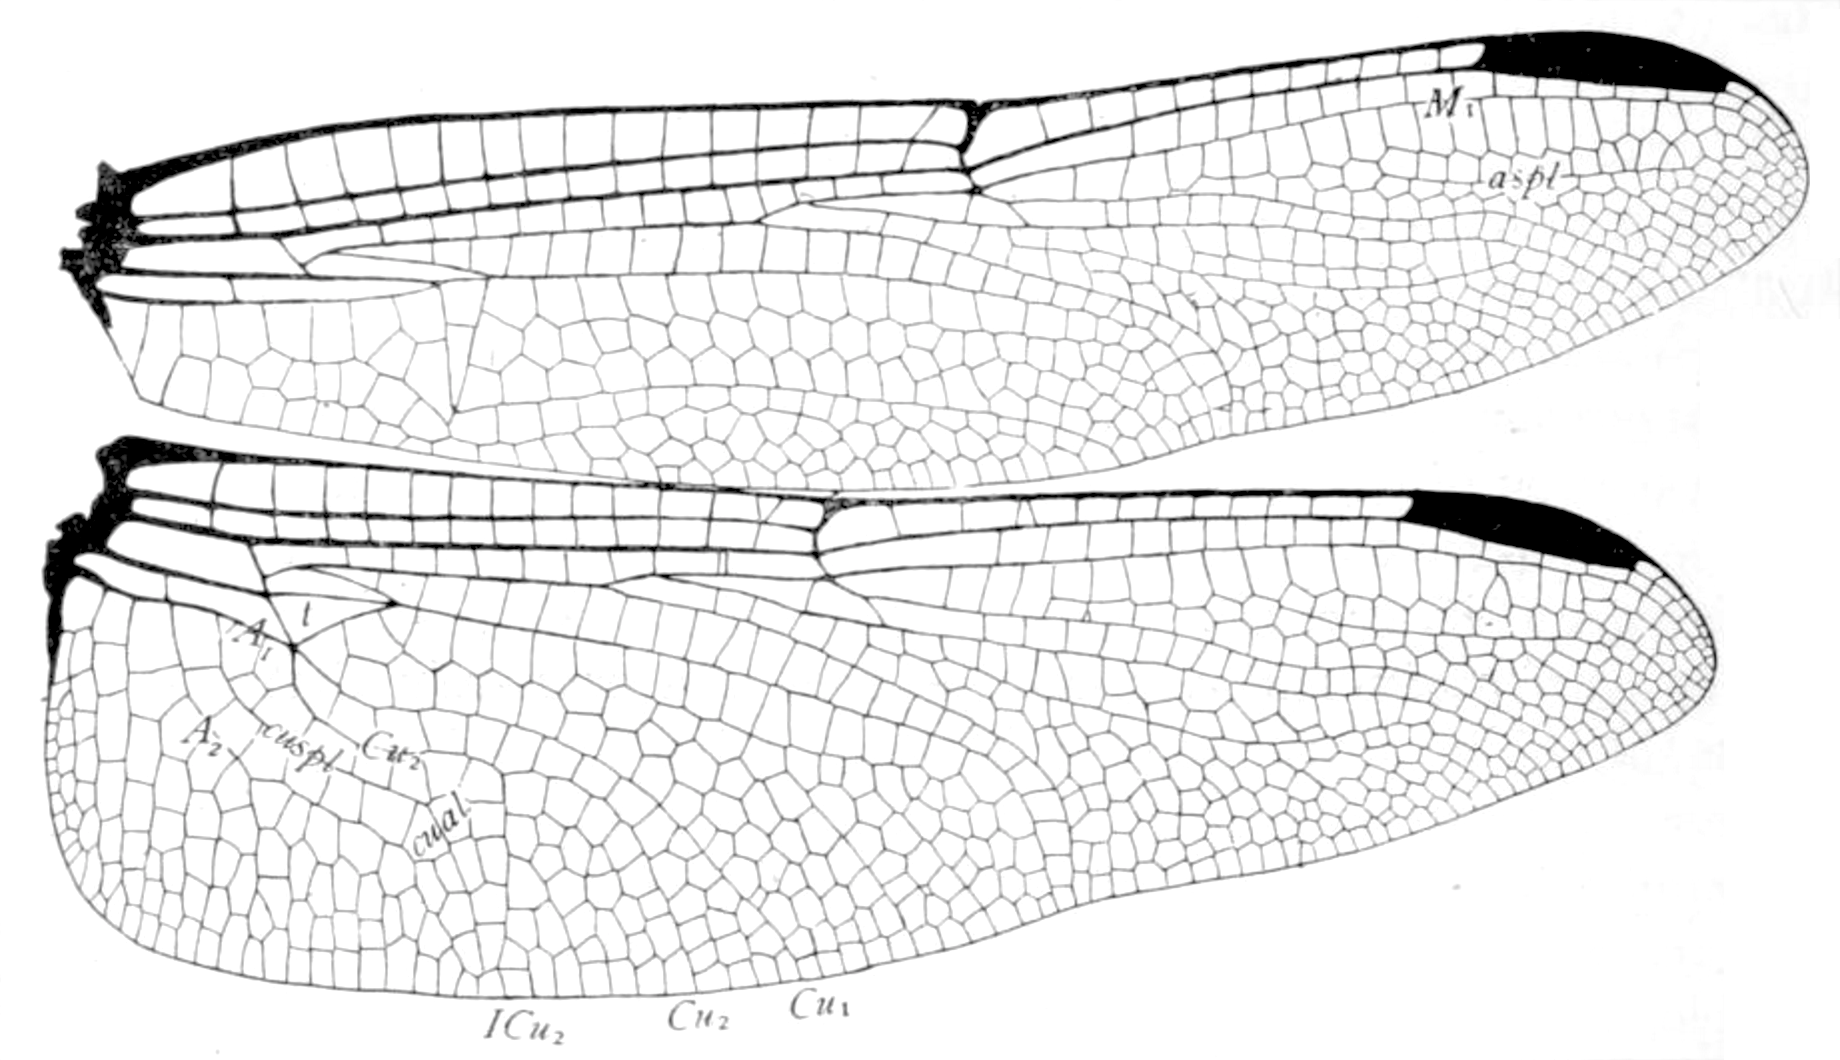
\includegraphics[width=\textwidth]{LibellulidWings}
        \caption{Wing venation \citep[][Fig. 240]{comstock1918wings}}
        \label{fig:libelwing}
    \end{subfigure}
    \hfill
    \begin{subfigure}[ht!]{0.45\textwidth}
        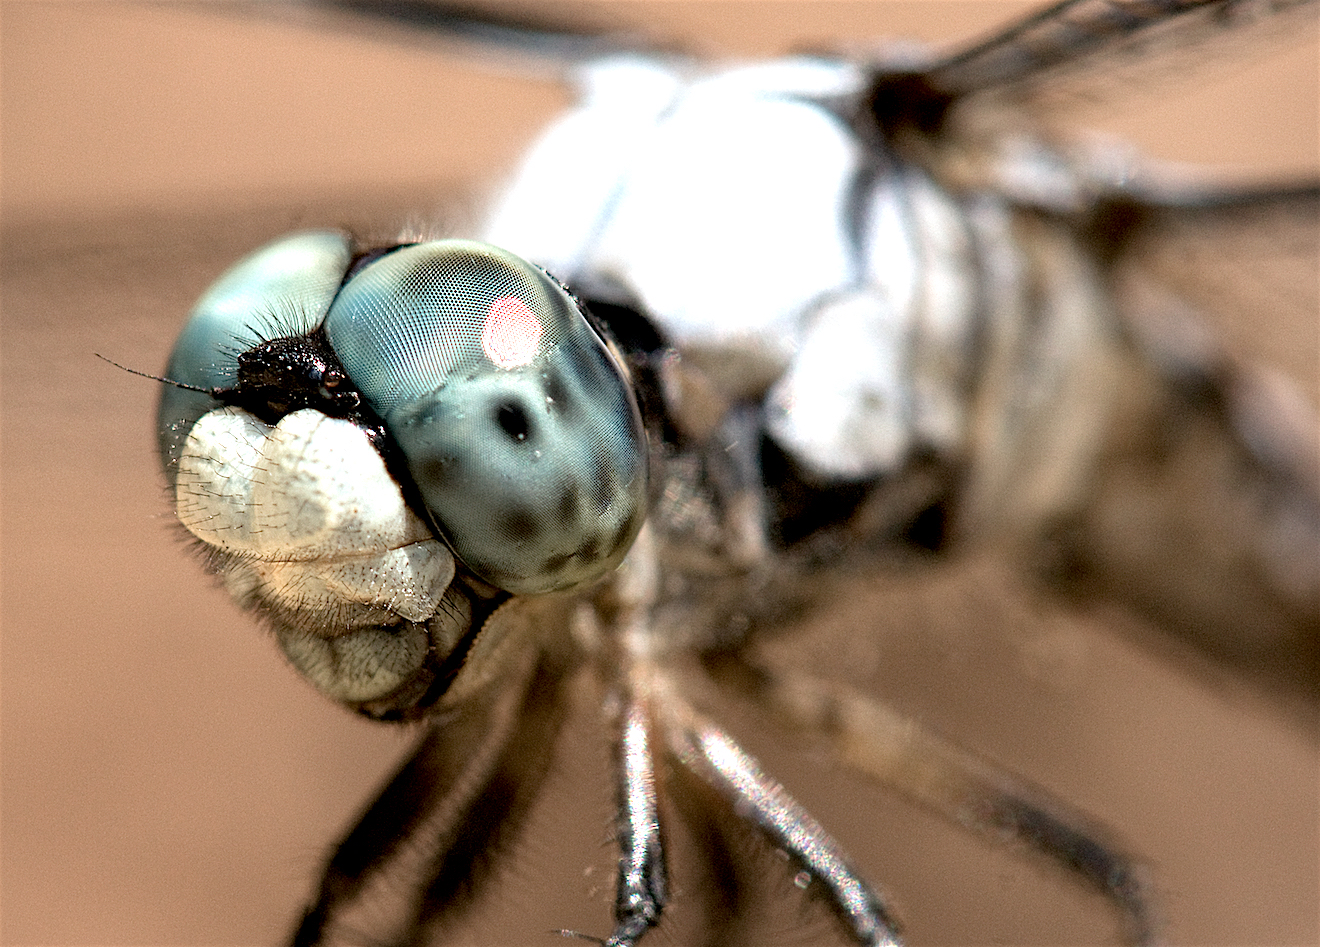
\includegraphics[width=\textwidth]{LibellulidHead}
        \caption{Head. Photo (CC BY-NC-SA 2.0) by e\_monk \url{https://flic.kr/p/8ua4sD}}
        \label{fig:libelbody}
    \end{subfigure}
    \caption{Libellulidae}\label{fig:libell}
\end{figure}

\subsection{Calopterygidae (jewelwings, broad-winged damselflies)}
\noindent{}\textit{Diagnostic characters:} Wings tapered at base, numerous antenodal crossveins present (proximal to nodus).\\

\noindent{}\textit{Natural history:} Like other damselflies, larvae are usually thought of as climbers. Larvae and adults are usually found along streams (\textit{i.e.}, lotic systems). Approximately 150 spp. have been described worldwide.\\

\begin{figure}[ht!]
    \centering
    \begin{subfigure}[ht!]{0.45\textwidth}
        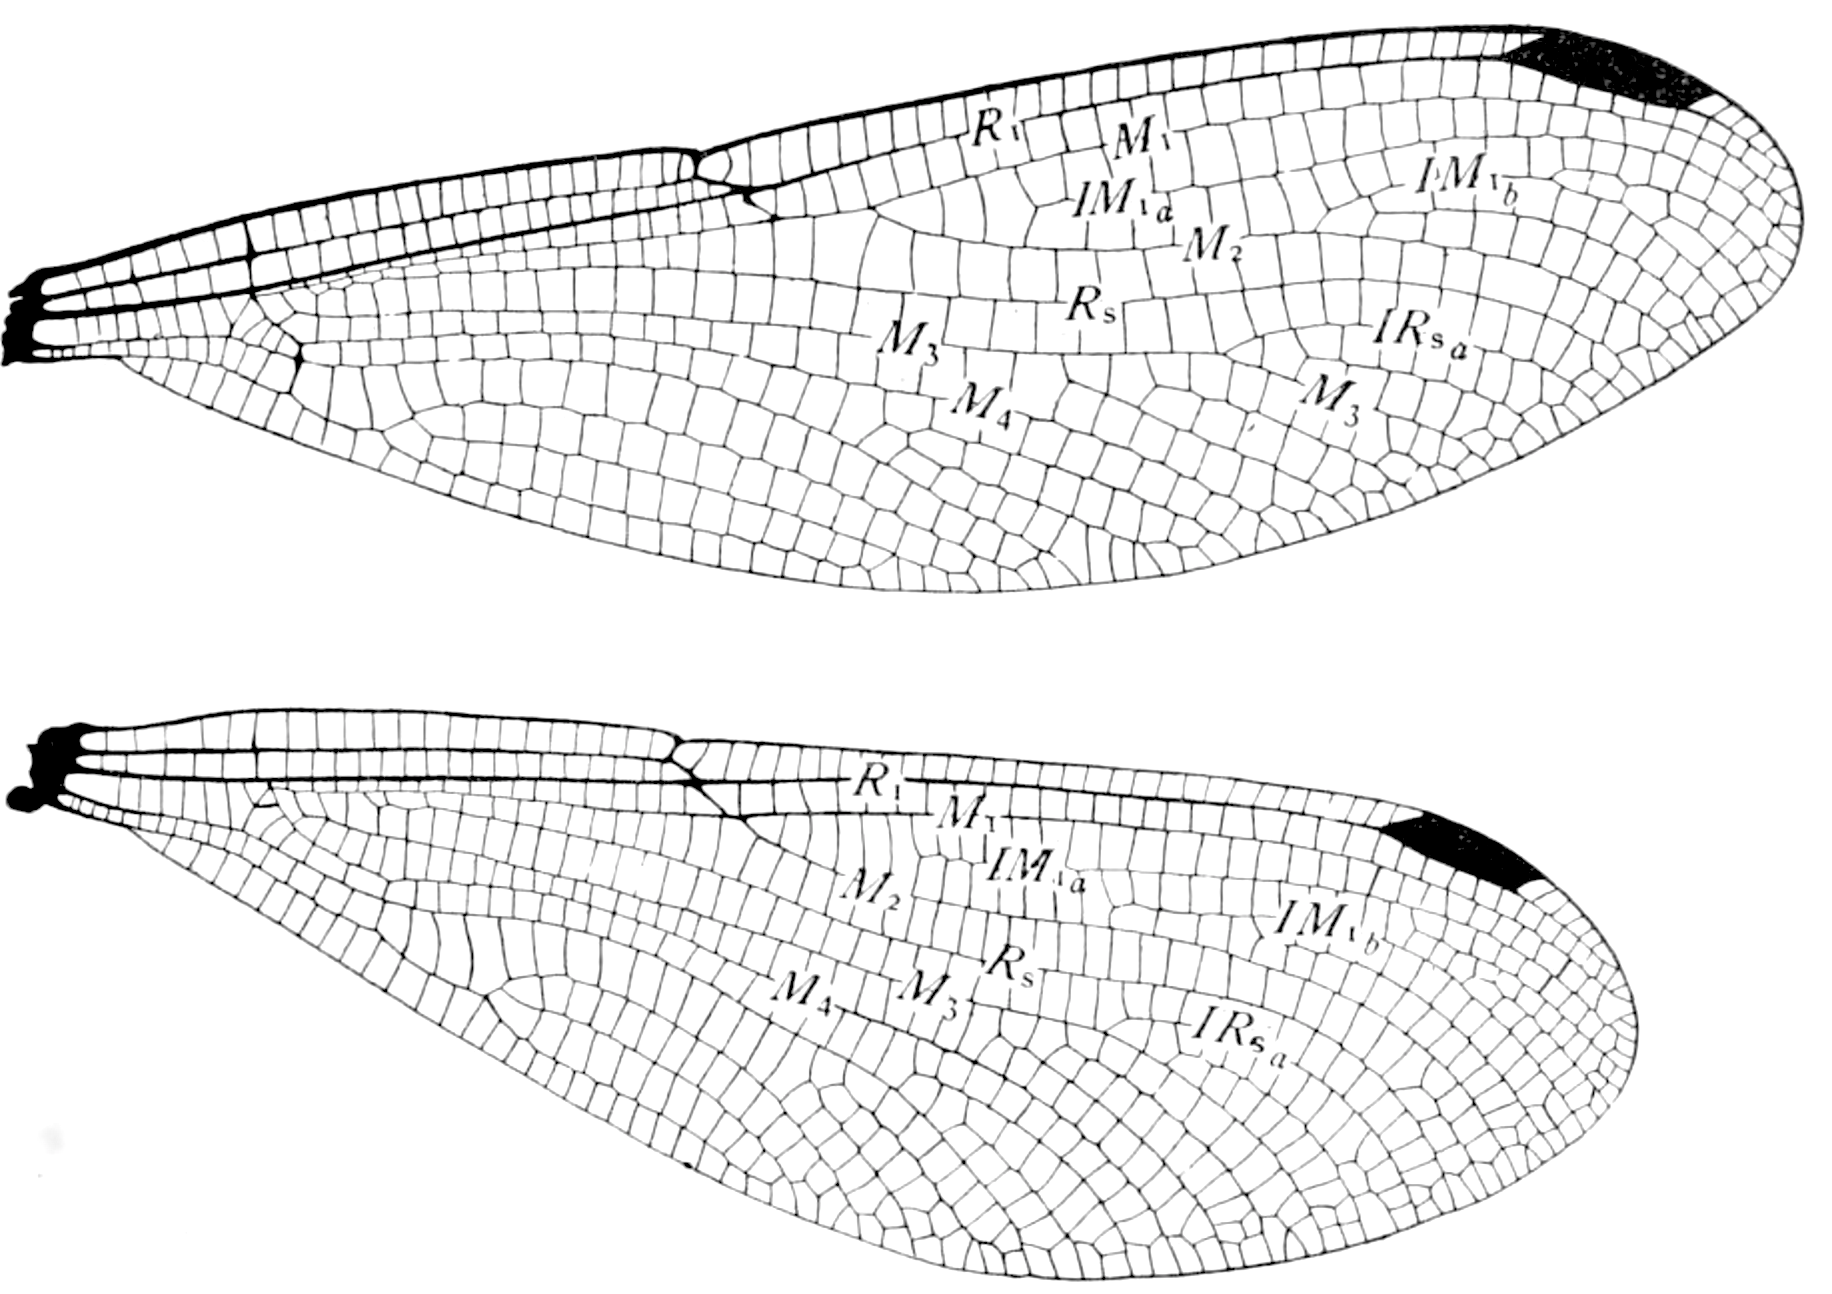
\includegraphics[width=\textwidth]{CalopterygidWing}
        \caption{Wing venation \citep[][Fig. 235]{comstock1918wings}}
        \label{fig:calopwing}
    \end{subfigure}
    \hfill
    \begin{subfigure}[ht!]{0.45\textwidth}
        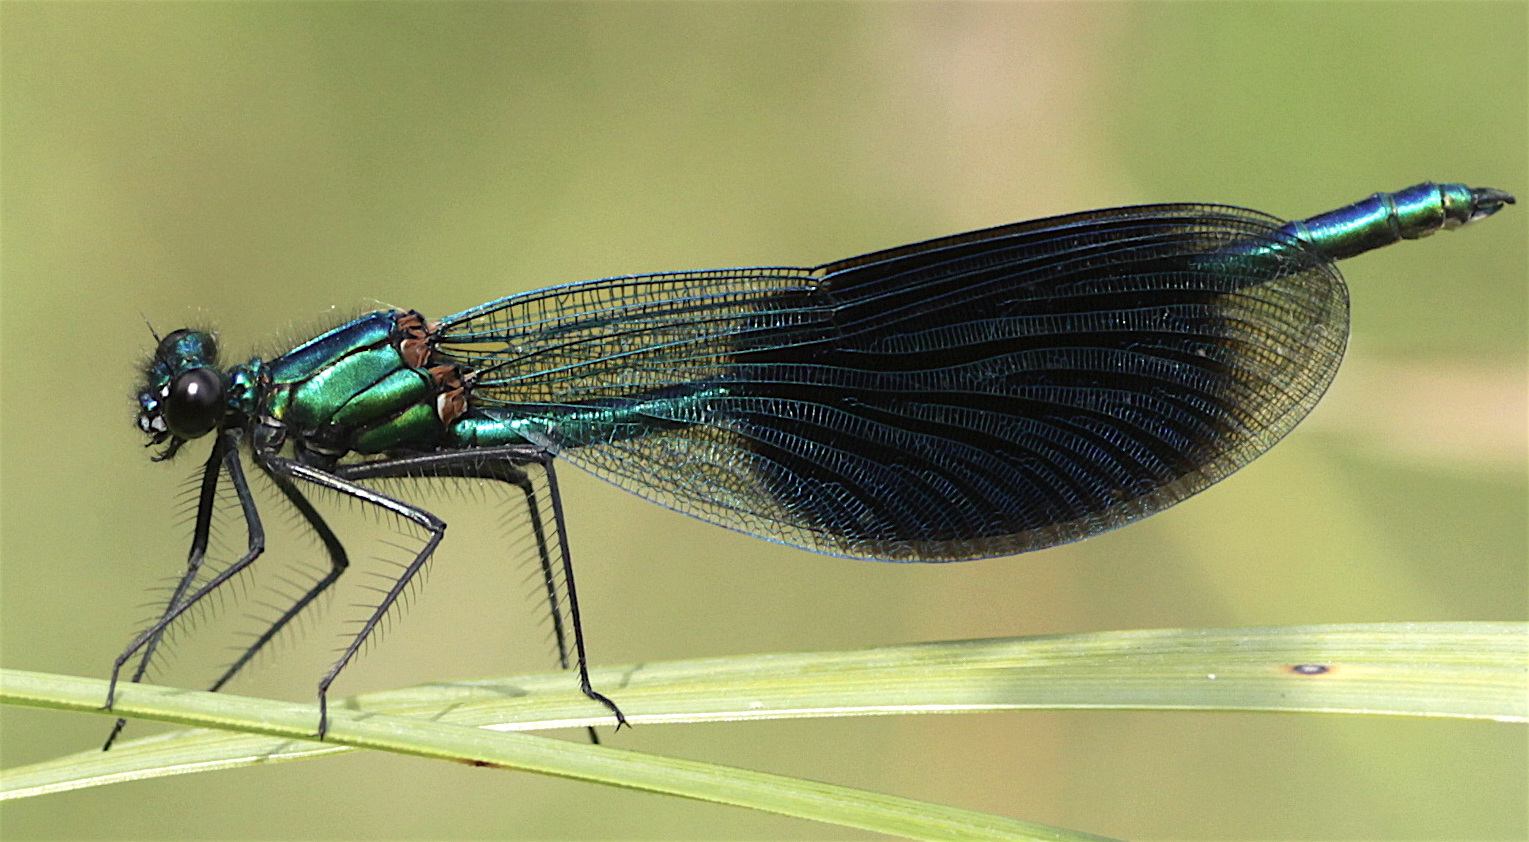
\includegraphics[width=\textwidth]{CalopterygidHabitus}
        \caption{Habitus. Photo (CC BY-NC-SA 2.0) by Mark Gurney \url{https://flic.kr/p/Cey6u8}}
        \label{fig:calopbody}
    \end{subfigure}
    \caption{Calopterygidae}\label{fig:calop}
\end{figure}

\subsection{Coenagrionidae (bluets, narrow-winged damselflies)}
\noindent{}\textit{Diagnostic characters:} wings stalked at base, few antenodal crossveins present, \texorpdfstring{M\textsubscript{3}}{ }{ } arises near nodus, quadrangle wing cell actually triangular.\\

\noindent{}\textit{Natural history:} Given the high level of diversity (\textgreater1,100 spp.), one can find these odonates in almost any aquatic habitat. Like other damselflies, larvae are usually thought of as climbers. Females oviposit in or near vegetation.\\

\begin{figure}[ht!]
    \centering
    \begin{subfigure}[ht!]{0.45\textwidth}
        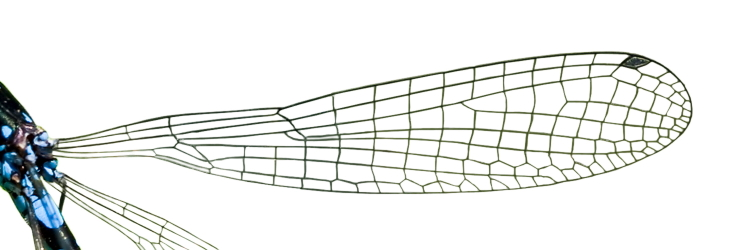
\includegraphics[width=\textwidth]{CoenagrionidWing}
        \caption{Fore wing. Photo (CC BY-SA 3.0) by L. B. Tettenborn \url{https://goo.gl/WLujq8}}
        \label{fig:coenwing}
    \end{subfigure}
    \hfill
    \begin{subfigure}[ht!]{0.45\textwidth}
        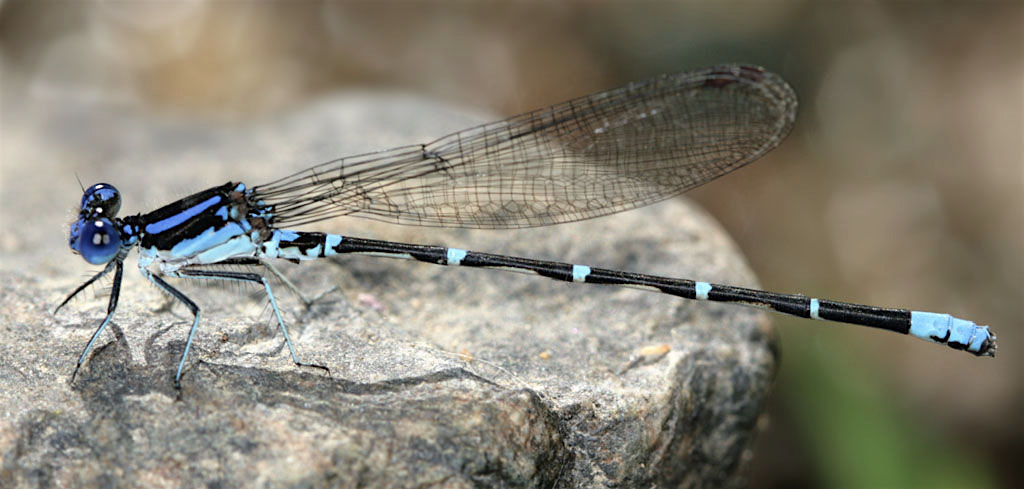
\includegraphics[width=\textwidth]{CoenagrionidHabitus}
        \caption{Habitus. Photo (CC BY-NC-SA 2.0) by Patrick Coin \url{https://flic.kr/p/2t47VF}}
        \label{fig:coenbody}
    \end{subfigure}
    \caption{Coenagrionidae}\label{fig:coenag}
\end{figure}

\subsection{Lestidae (spreadwings)}
\noindent{}\textit{Diagnostic characters:} wings stalked at base, few antenodal crossveins present, \texorpdfstring{M\textsubscript{3}}{ }{ } arises near arculus, quadrangle wing cell actually quadrangular. \\

\noindent{}\textit{Natural history:} Naiads are found in a variety of aquatic environments and have a distinctive, elongate habitus and a spoon-like labium. Unlike other damselflies, adult lestids usually rest on vegetation with their wings at least partially spread. Approximately 150 spp. have been described worldwide.\\ 

\begin{figure}[ht!]
    \centering
    \begin{subfigure}[ht!]{0.45\textwidth}
        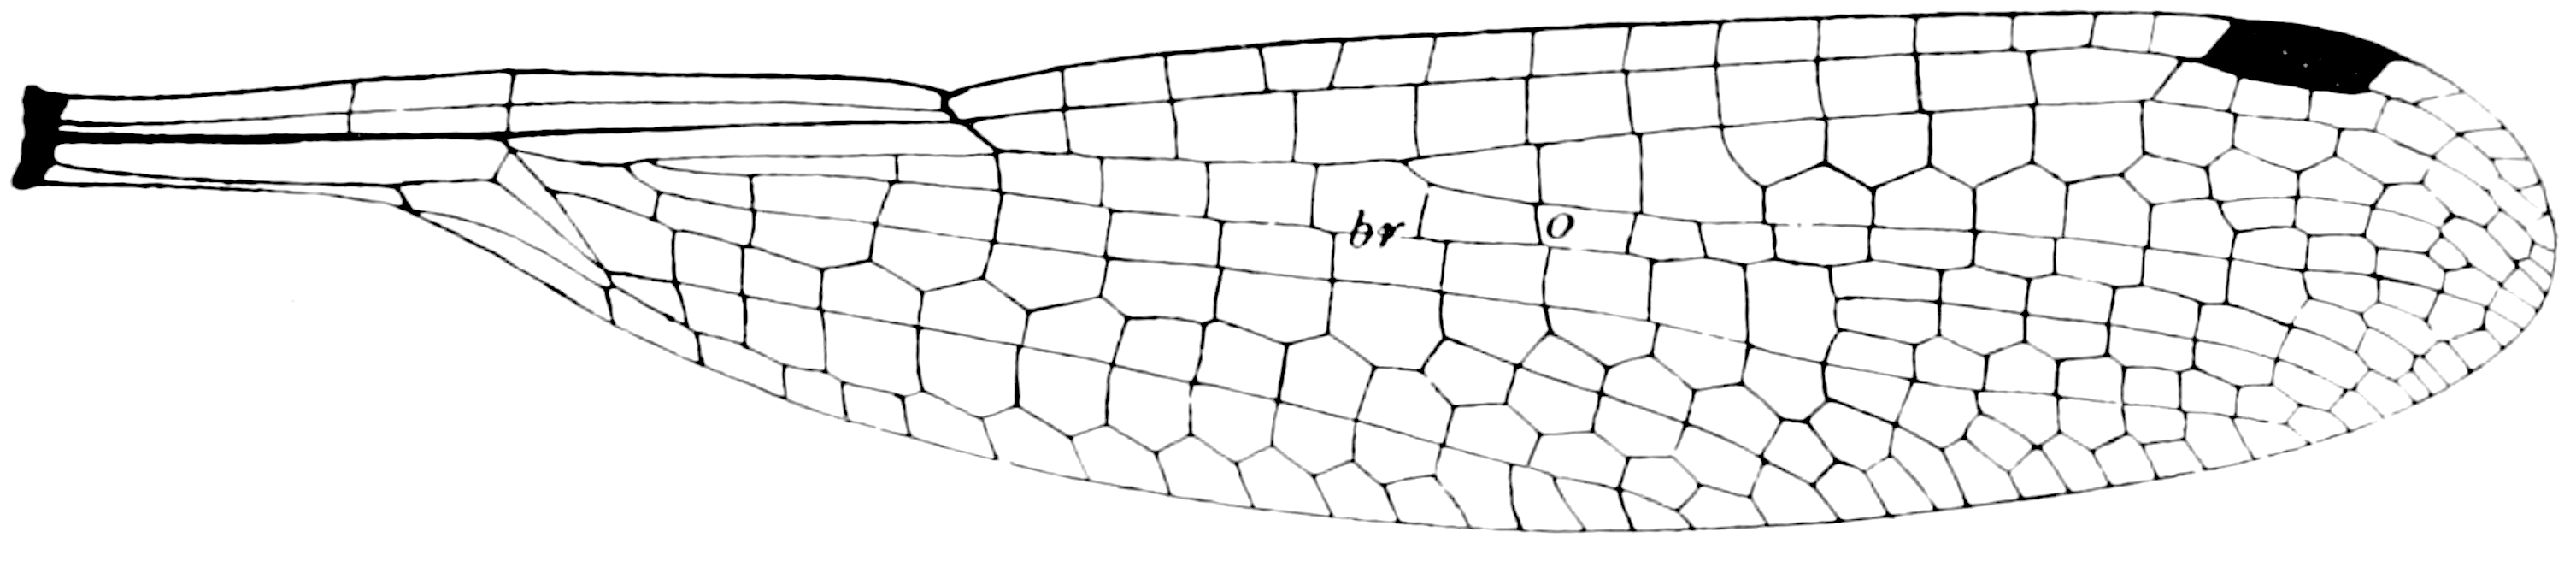
\includegraphics[width=\textwidth]{LestidWing}
        \caption{Wing venation \citep[][Fig. 232]{comstock1918wings}}
        \label{fig:lestwing}
    \end{subfigure}
    \hfill
    \begin{subfigure}[ht!]{0.45\textwidth}
        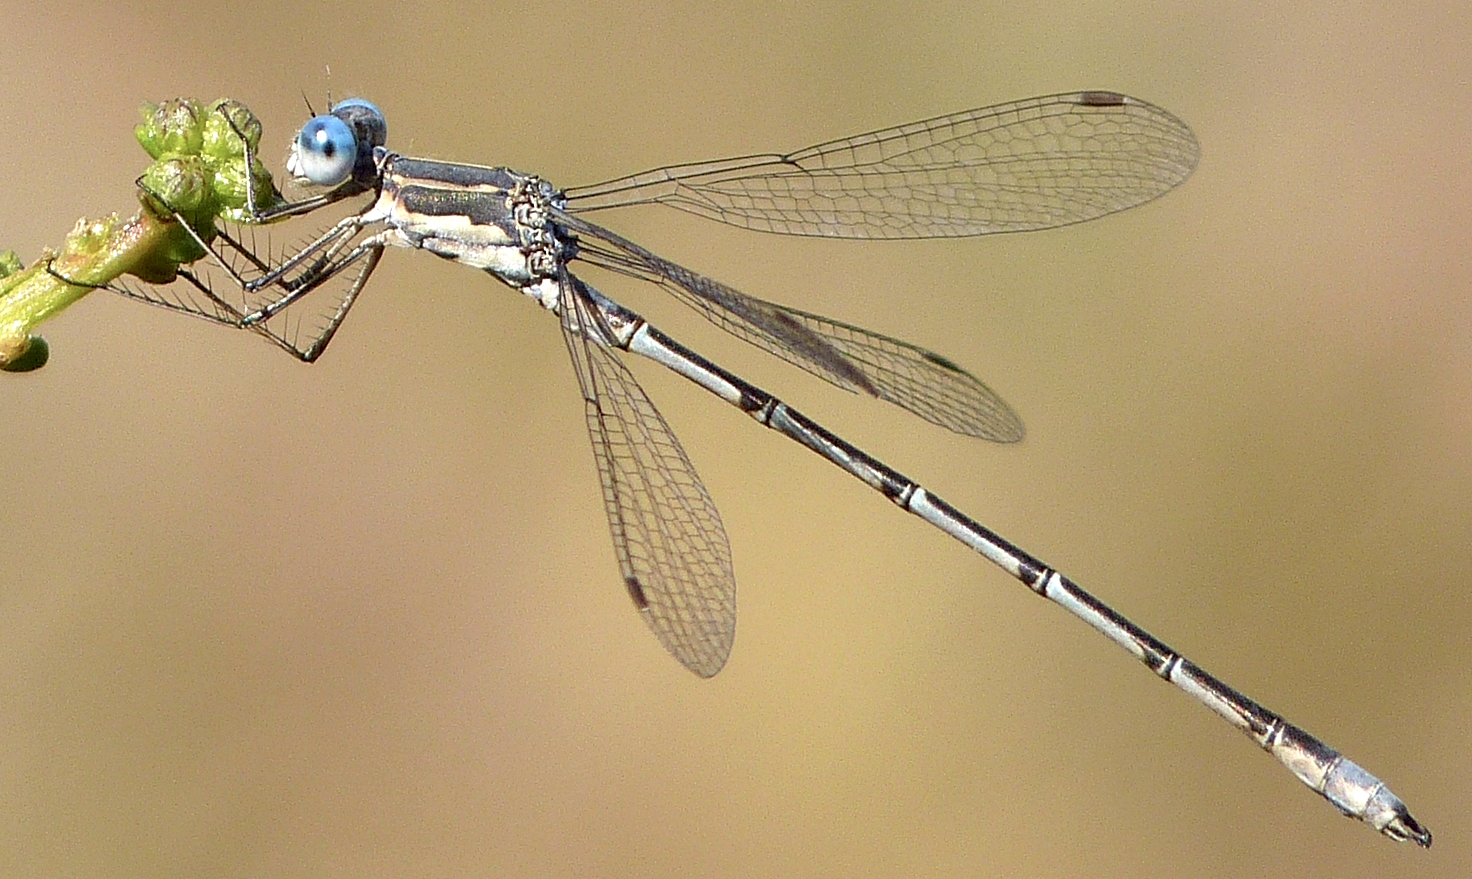
\includegraphics[width=\textwidth]{LestidHabitus}
        \caption{Habitus. Photo (CC BY-NC 2.0) by Mathesont \url{https://flic.kr/p/d3aZu3}}
        \label{fig:lestbody}
    \end{subfigure}
    \caption{Lestidae}\label{fig:lestid}
\end{figure}

\subsection*{Naiads}
Take a moment to observe Odonata naiads of several families under your microscope. \\

\hangindent2em\textbf{Question 7-7:} Can you find two larval adaptations for predation?\\

\hangindent2em\textbf{Question 7-8:} What morphological differences to you see between a dragonfly naiad and a damselfly naiad? Make a sketch.

\begin{figure}[ht!]
  \centering
    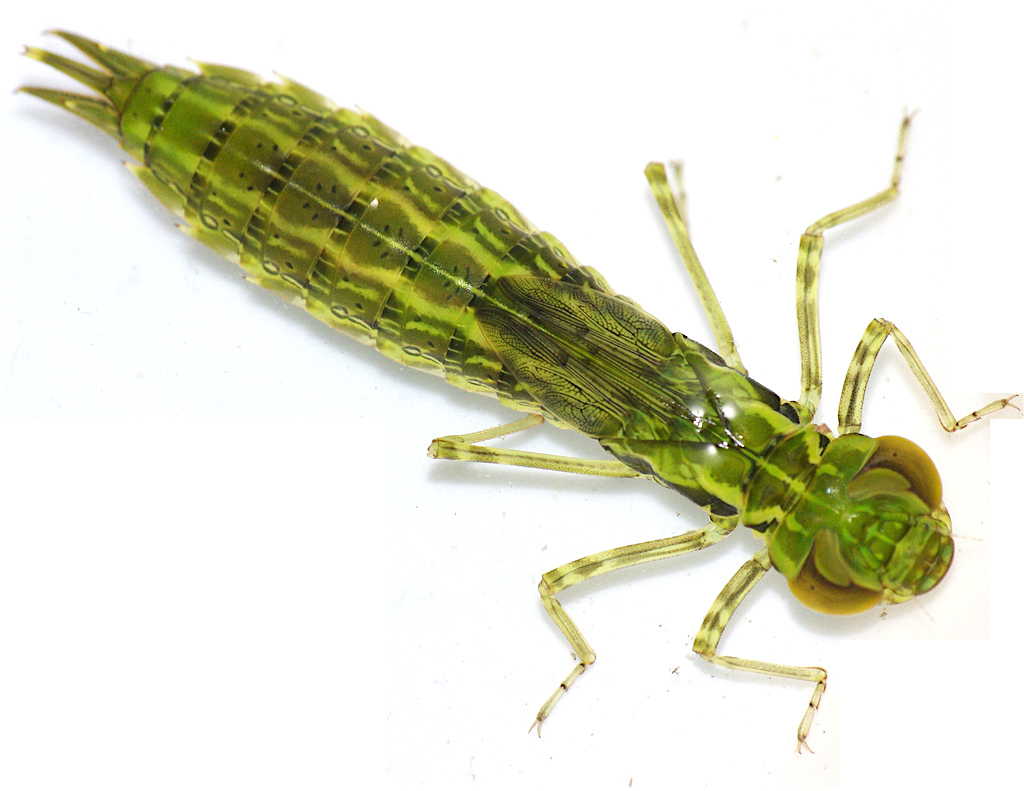
\includegraphics[width=0.45\textwidth]{AeshnidLarva}
  \caption{Aeshnidae. Photo (CC BY-NC 2.5) by Brad Carlson \url{https://flic.kr/p/bLjCAp}}
  \label{fig:OdonataLarva}
\end{figure}

\FloatBarrier

\section*{Pterygota: Neoptera}
The remaining insect orders are classified in Neoptera, a lineage whose members can pull their wings over their abdomens when they're at rest. This movement is accomplished by flexing a pleural muscle that inserts on the 3rd axillary sclerite. The wing then folds along flexion lines that are not present in Palaeoptera, allowing the wing to be pulled back posteriorly.\\

\hangindent2em\textbf{Question 7-9:} In this unit we've touched on two evolutionary events that are considered to be \textit{key innovations}: the origin of wings and the the origin of neoptery. Why do you think these two adaptations led to explosive diversification?

\section{Plecoptera (stoneflies)}
Like the previous two orders, Plecoptera are aquatic during their immature stages and semi-aquatic/terrestrial as adults. More than 100 million years of evolution probably separates Plecoptera from Odonata and Ephemeroptera \citep{Misof763}, so stoneflies are not closely related (relatively speaking) to dragonflies and mayflies. It is useful to treat them here, however, as they have similar habits to mayflies, are important for monitoring water quality (like Ephemeroptera), and have inspired much speculation on the origin of wings.

\subsection*{Naiads}
Stonefly naiads are almost exclusively found in lotic environments---\textit{e.g.}, clear, clean, highly oxygenated streams---and they are generally very sensitive to water quality. The immature stages develop as predators of other aquatic invertebrates or as shredders of vegetative material. They can be recognized from other aquatic non-holometabolous insects by (a) the presence of two tarsal claws on each leg and (b) two cerci on the apex of the abdomen.

\noindent{}Select specimens of at least three families and look for phenotypic differences in these diagnostic traits:
\begin{itemize}
\item presence/absence of gill tufts on the thorax and/or abdomen
\item width and shape of nota in dorsal view
\end{itemize}

\subsection*{Adults}
Stoneflies are generally not good dispersers and so are found near the features from which their naiads emerged. The diagnostic features can be subtle, so it's important to spend some time understanding the relevant morphology:

\begin{itemize}
\item Glossa length relative to paraglossa length (\textit{cf}.\footnote{From the Latin verb \textit{conferre}, to bring together, used here to invite the reader to compare the listed taxa.} Perlidae or Perlodidae \textit{vs}. Leuctridae or Capniidae)
\item Presence/location of gill remnants (\textit{cf}. Perlidae \textit{vs}. Perlodidae. Hint: look near the coxae)
\item Wing phenotype at rest (\textit{cf}. Perlidae or Perlodidae \textit{vs}. Leuctridae)
\item (wing venation!)%add these
\item Relative length of the cerci (\textit{cf}. Perlidae or Perlodidae \textit{vs}. Leuctridae)
\end{itemize}

\subsection{Perlidae (common stoneflies)}
\noindent{}\textit{Diagnostic characters:} Glossae much shorter than paraglossae, cercus longer than pronotum width, branched gill remnants present behind leg bases, , fore wing not rolled around body

\noindent{}\textit{Natural history:} \\ 

\begin{figure}[ht!]
    \centering
    \begin{subfigure}[ht!]{0.45\textwidth}
        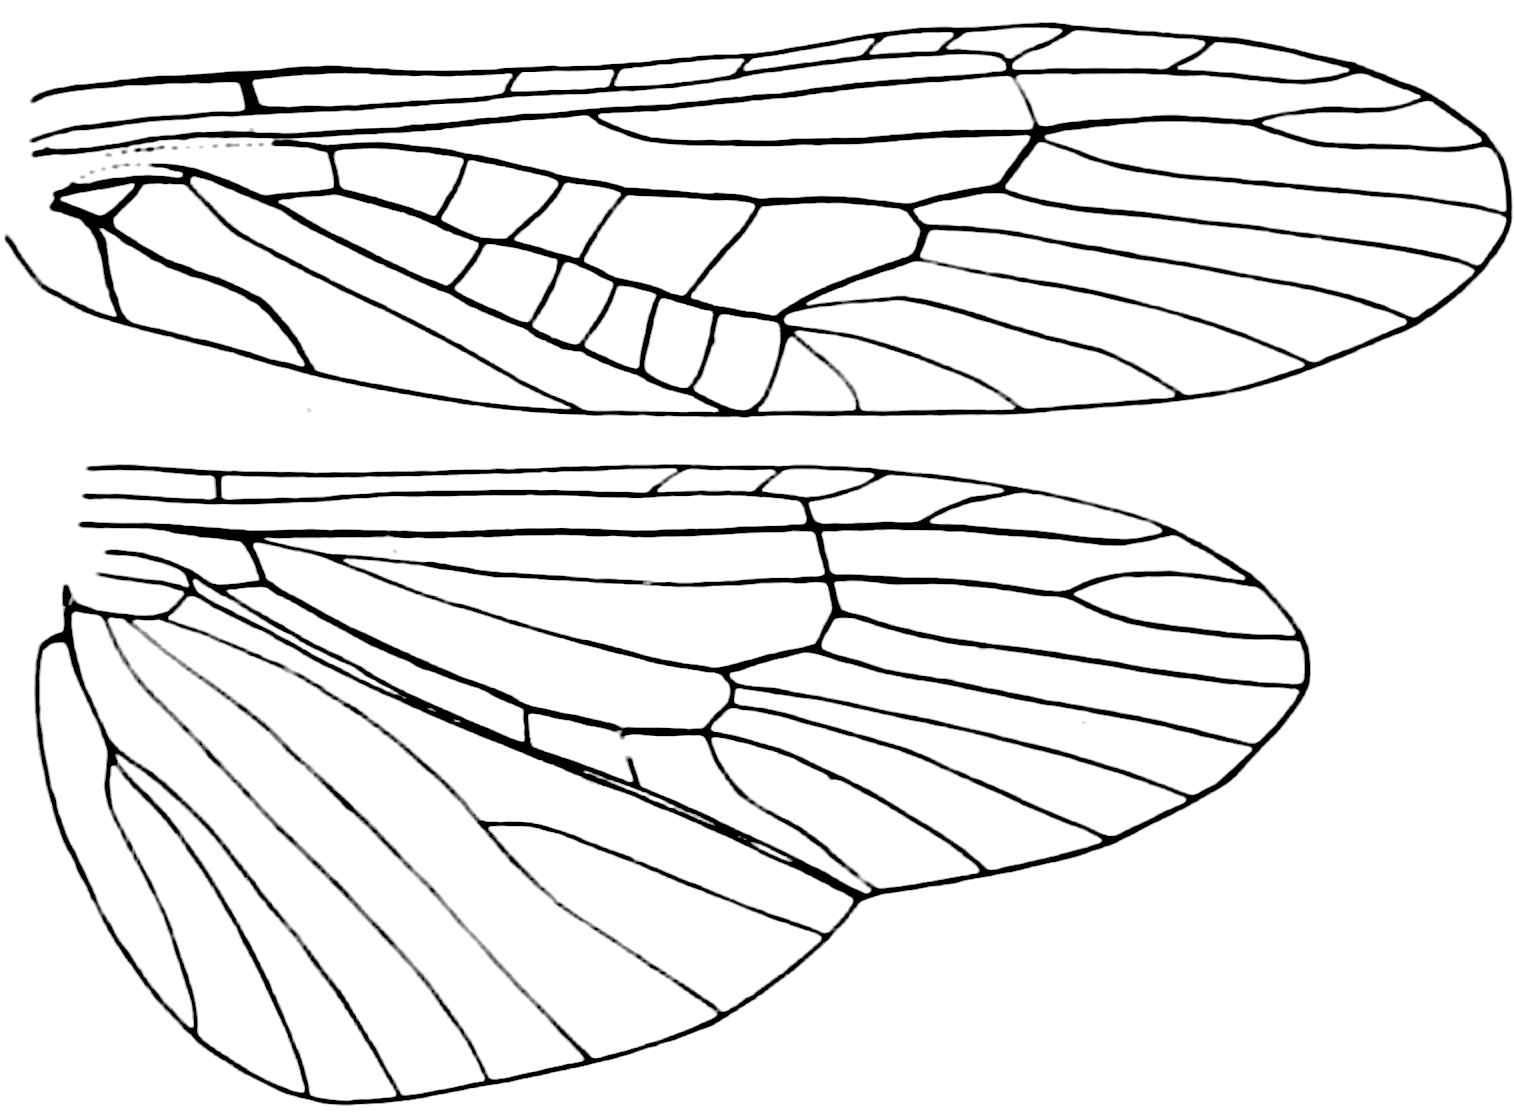
\includegraphics[width=\textwidth]{PerlidWings}
        \caption{Wings \citep[modified from][Plate 11, Fig. 3]{bhl29875}}
        \label{fig:perlid1}
    \end{subfigure}
    \qquad
    \begin{subfigure}[ht!]{0.45\textwidth}
        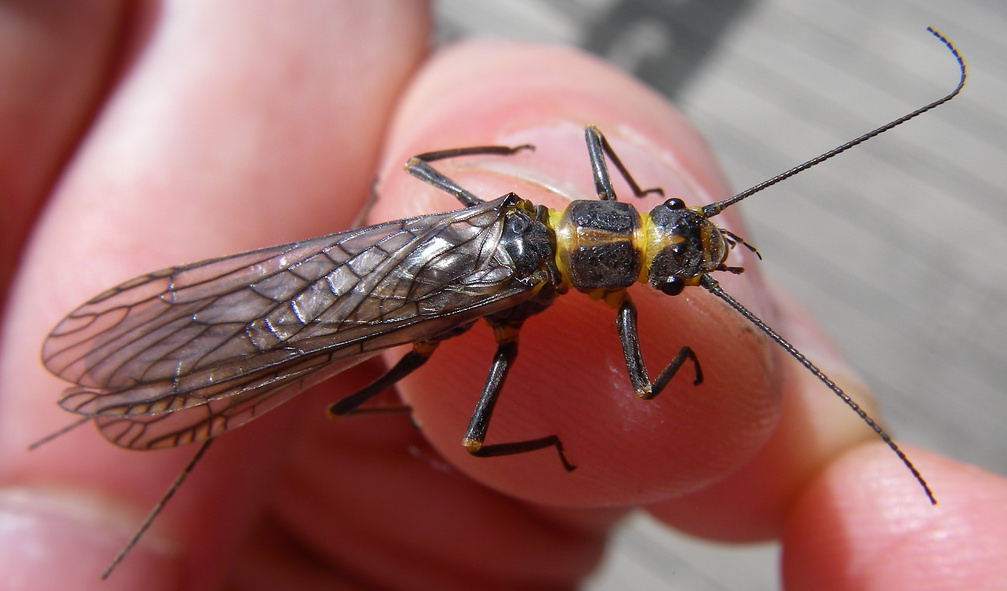
\includegraphics[width=\textwidth]{perlid}
        \caption{Perlidae. Photo (CC BY-SA 2.0) by Jerry Schoen \url{https://flic.kr/p/o3rdmk}}
        \label{fig:perlid2}
    \end{subfigure}
    \caption{Perlidae}\label{fig:perlids}
\end{figure}

\subsection{Perlodidae}
\noindent{}\textit{Diagnostic characters:} Glossae much shorter than paraglossae, cercus longer than pronotum width, branched gill remnants absent, cubito-anal crossvein arising distal to anal cell, 4 or more Cu crossveins on fore wing, 2A forked, fore wing not rolled around body.\\

\noindent{}\textit{Natural history:} .\\

\begin{figure}[ht!]
    \centering
    \begin{subfigure}[ht!]{0.4\textwidth}
        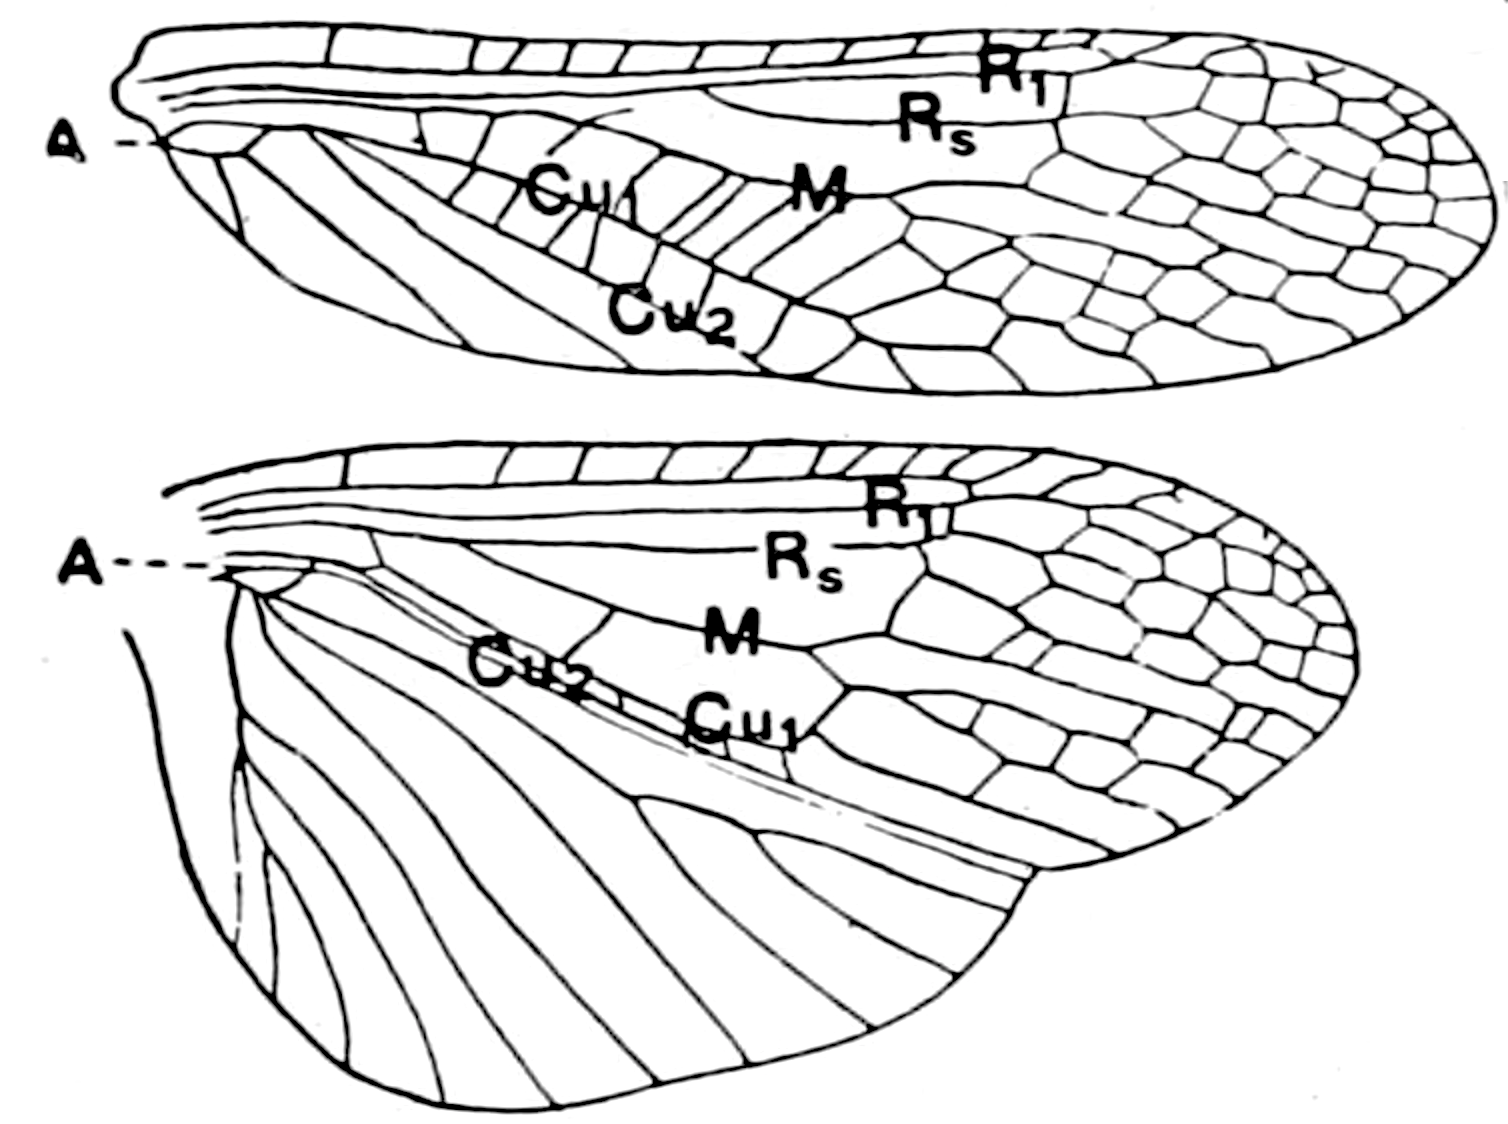
\includegraphics[width=\textwidth]{PerlodidWings}
        \caption{Wings \citep[modified from][Plate 9, Fig. 1]{bhl29875}}
        \label{fig:perlodid1}
    \end{subfigure}
    \qquad
    \begin{subfigure}[ht!]{0.5\textwidth}
        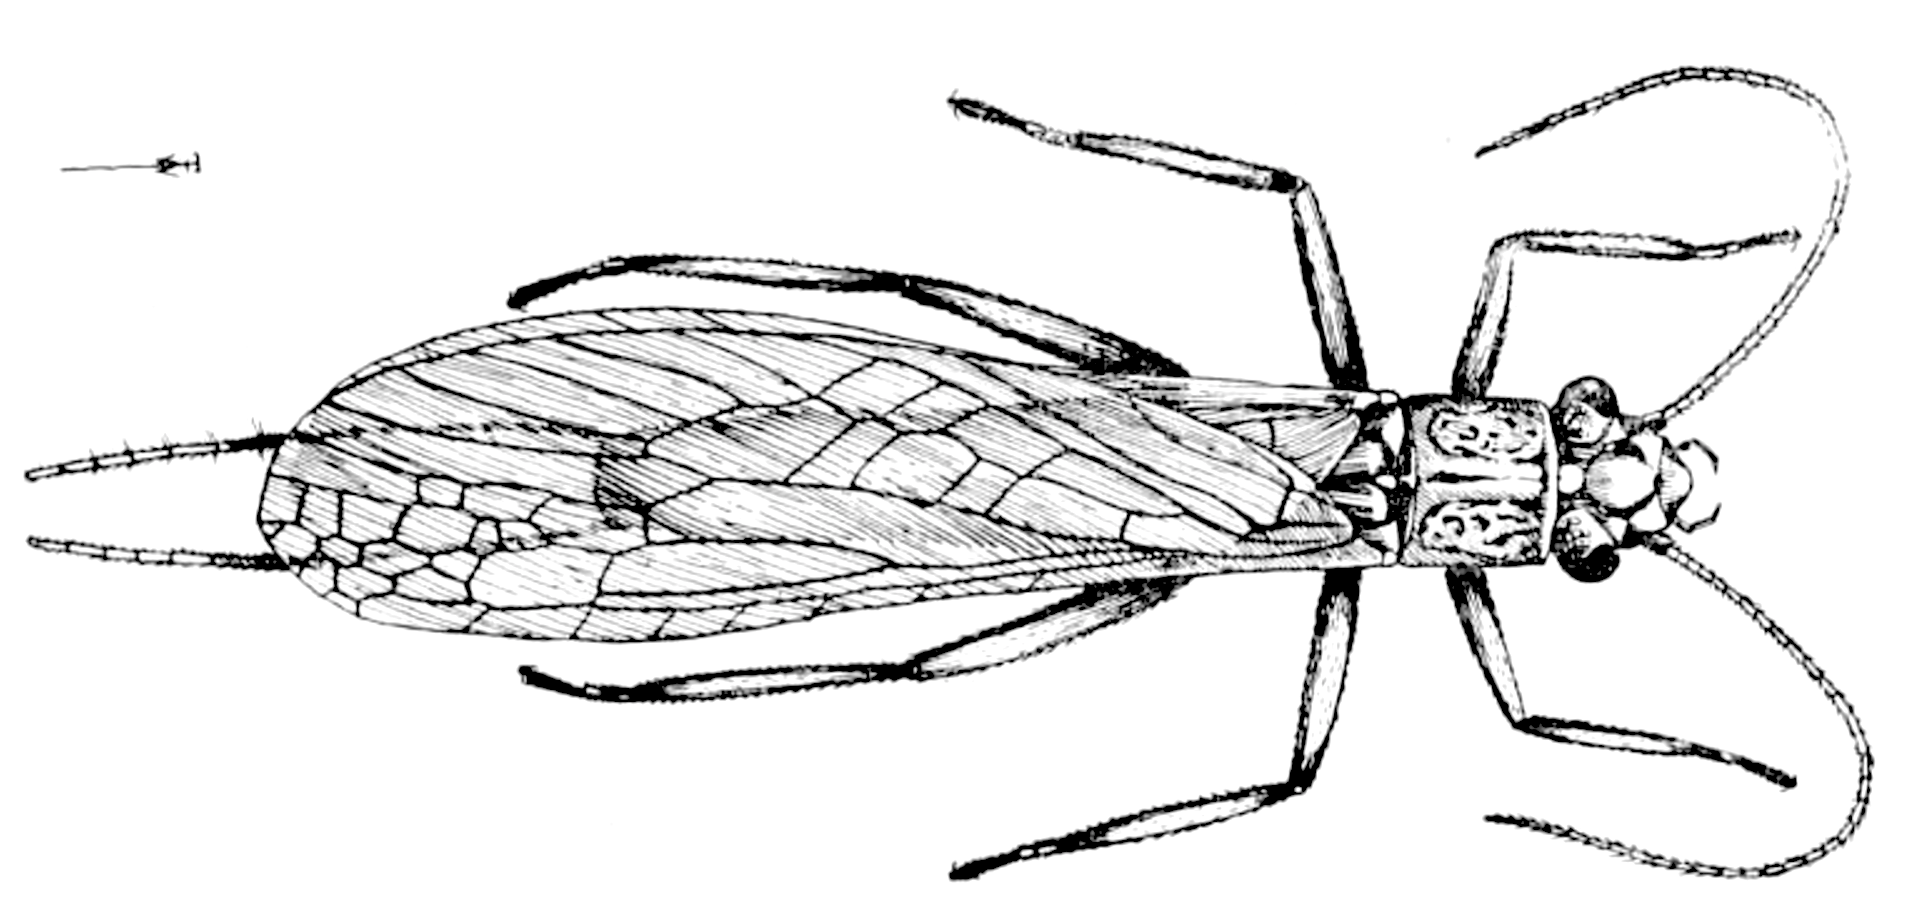
\includegraphics[width=\textwidth]{PerlodidHabitus}
        \caption{Wings \citep[modified from][Fig. 12]{bhl29875}}
        \label{fig:perlodid2}
    \end{subfigure}
    \caption{Perlodidae}\label{fig:perlodids}
\end{figure}

\subsection{Leuctridae (rolled-wing stoneflies)}%delete?
\noindent{}\textit{Diagnostic characters:} Glossae same length as paraglossae, cercus very short composed of one segment, branched gill remnants absent, cubito-anal crossvein arising distal to or from anal cell, 4 or more Cu crossveins on fore wing; 2A forked, fore wings rolled around body.\\

\noindent{}\textit{Natural history:} .\\

\begin{figure}[ht!]
    \centering
    \begin{subfigure}[ht!]{0.4\textwidth}
        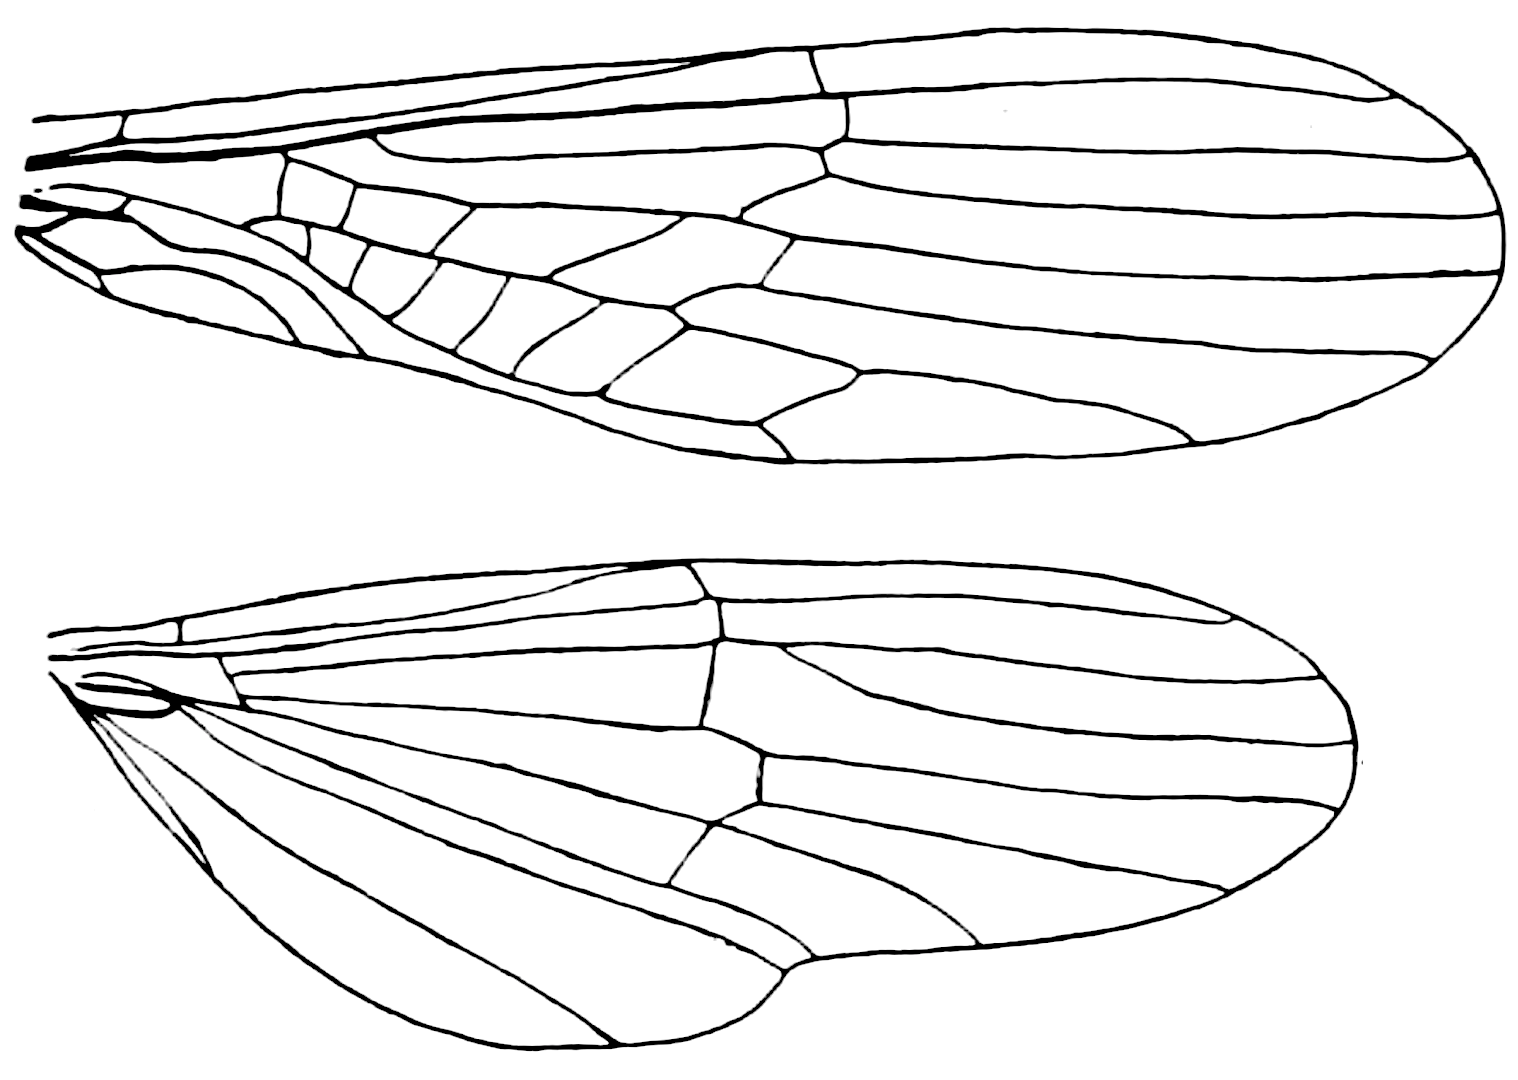
\includegraphics[width=\textwidth]{LeuctridWings}
        \caption{Wings \citep[modified from][Plate 32, Fig. 1]{bhl29875}}
        \label{fig:leuctrid1}
    \end{subfigure}
    \qquad
    \begin{subfigure}[ht!]{0.5\textwidth}
        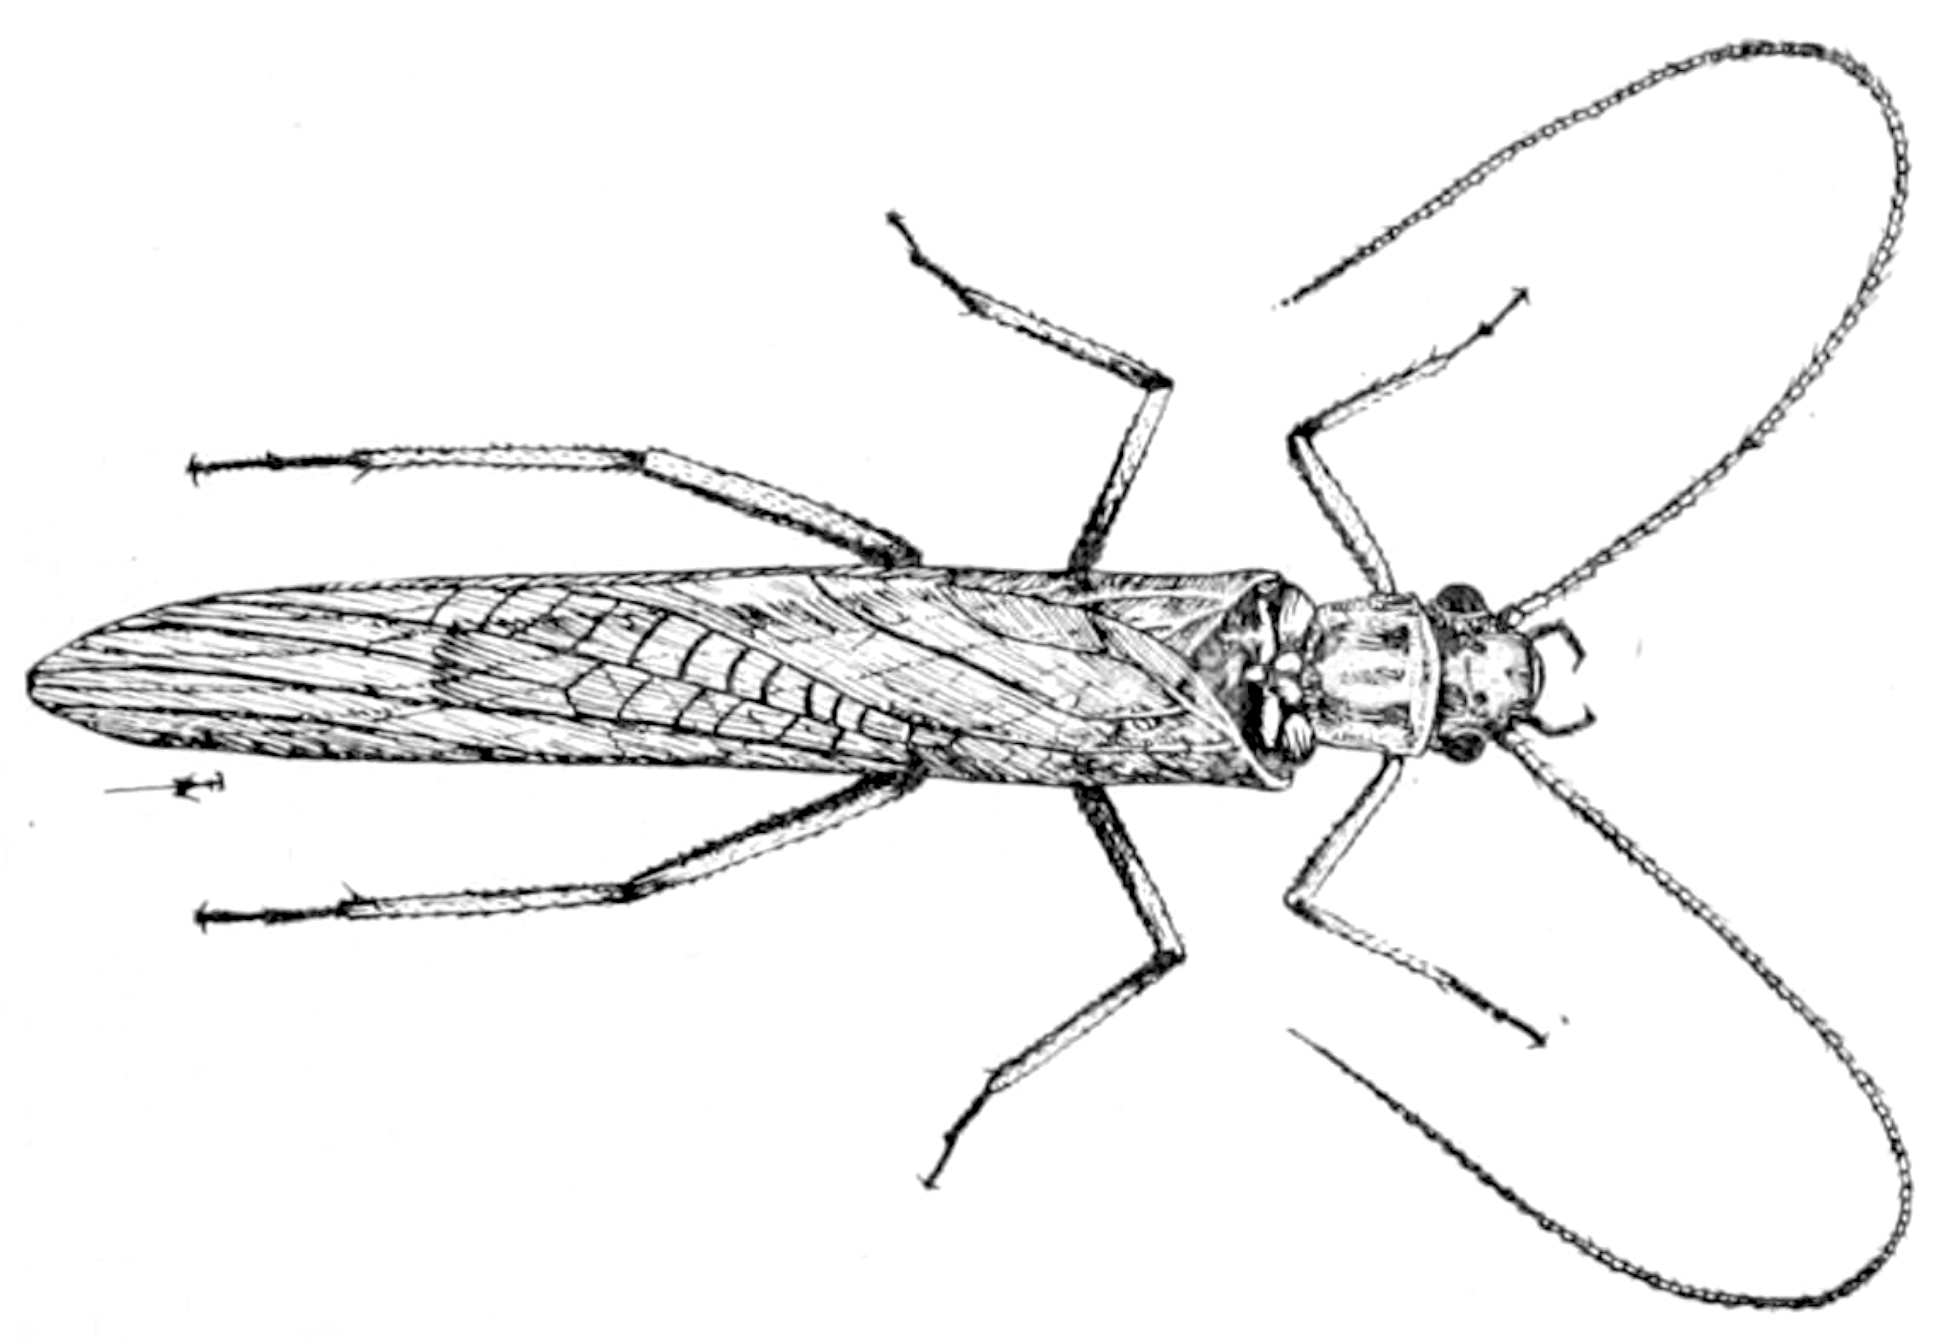
\includegraphics[width=\textwidth]{LeuctridHabitus}
        \caption{Wings \citep[modified from][Fig. 26]{bhl29875}}
        \label{fig:leuctrid2}
    \end{subfigure}
    \caption{Perlodidae}\label{fig:leuctrids}
\end{figure}

\subsection{Capniidae (winter stoneflies)}
\noindent{}\textit{Diagnostic characters:} Glossae same length as paraglossae, cercus with at least 4 segments, gill remnants absent, cubito-anal crossvein arising distal to or from anal cell, 1--2 or more Cu crossveins on fore wing, 2A not forked.\\

\noindent{}\textit{Natural history:} .\\

\begin{figure}[ht!]
    \centering
    \begin{subfigure}[ht!]{0.4\textwidth}
        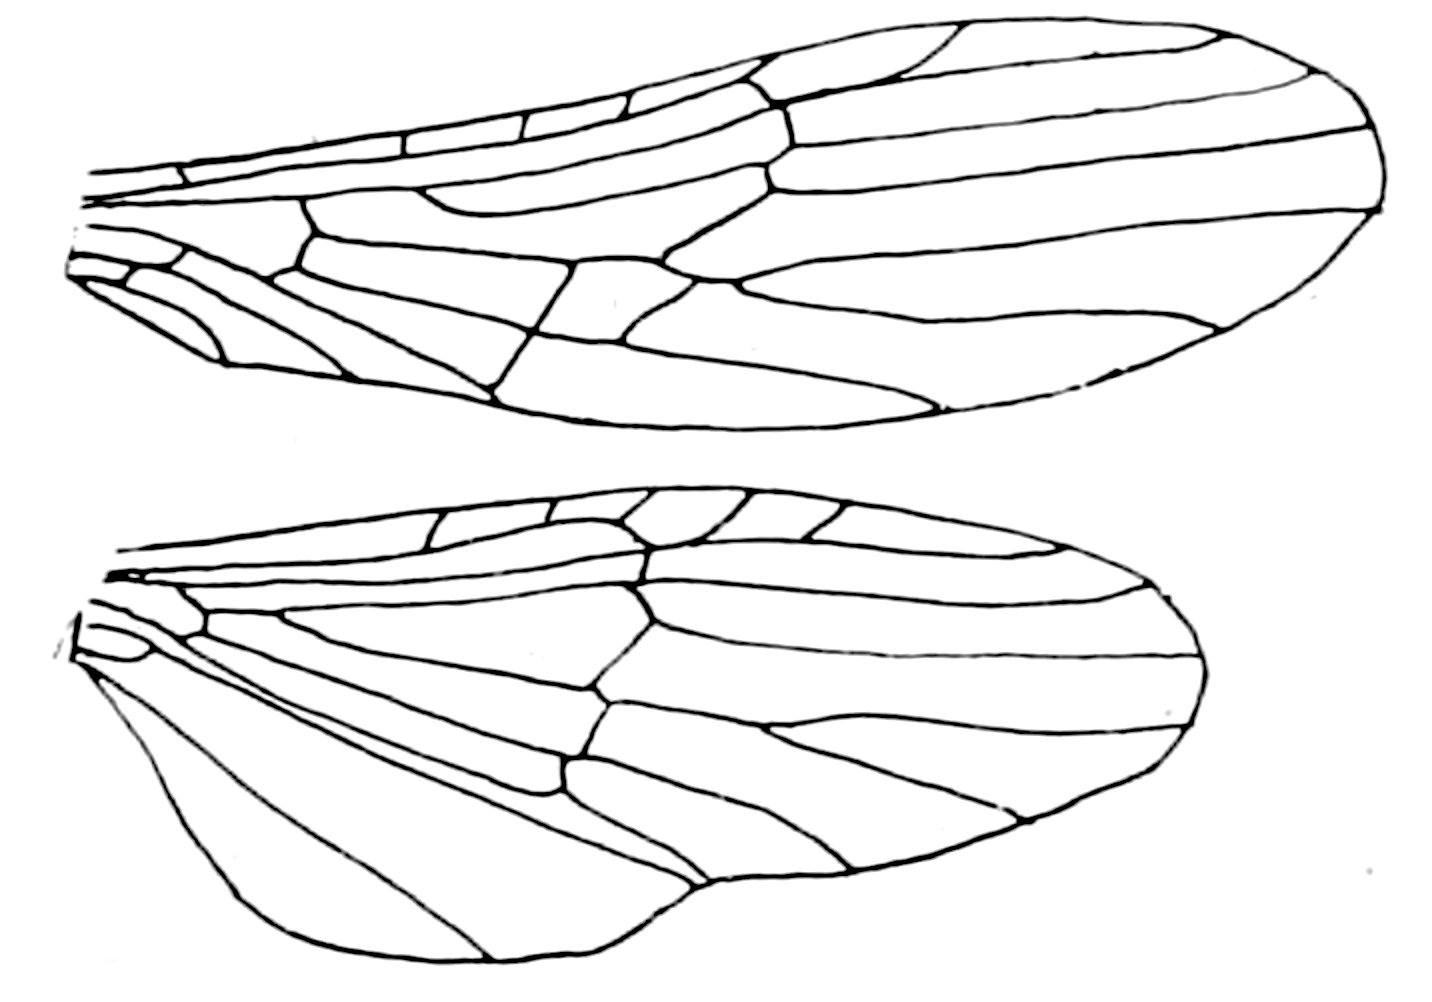
\includegraphics[width=\textwidth]{CapniidWings}
        \caption{Wings \citep[modified from][Plate 47, Fig. 2]{bhl29875}}
        \label{fig:capniid1}
    \end{subfigure}
    \qquad
    \begin{subfigure}[ht!]{0.5\textwidth}
        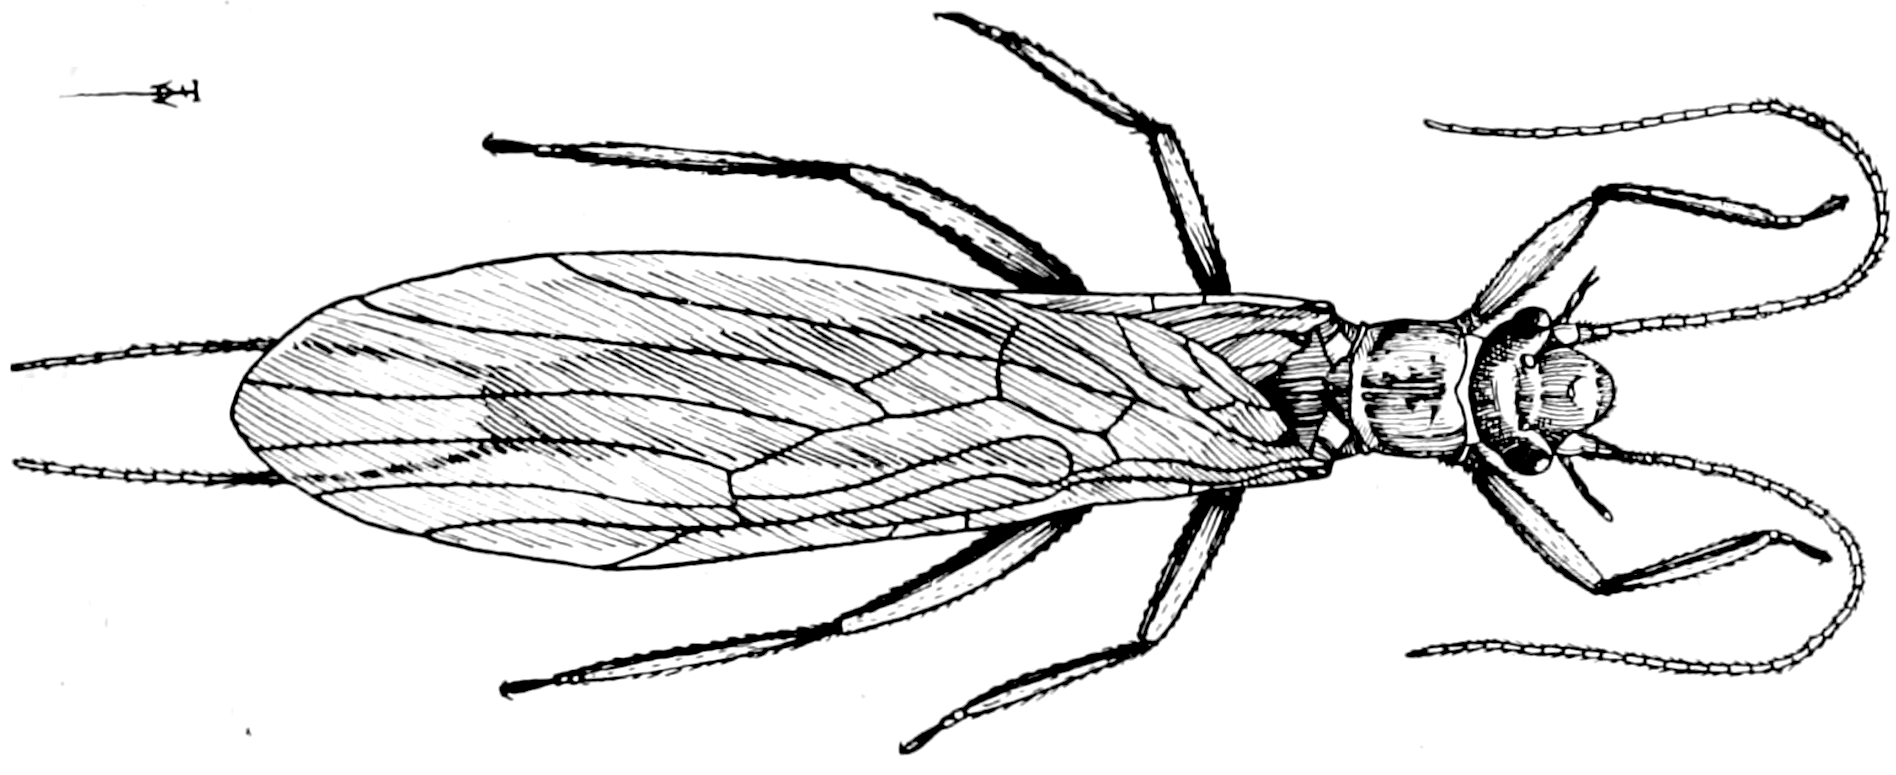
\includegraphics[width=\textwidth]{CapniidHabitus}
        \caption{Habitus \citep[modified from][Fig. 28]{bhl29875}}
        \label{fig:capniid2}
    \end{subfigure}
    \caption{Capniidae}\label{fig:capniids}
\end{figure}

\section*{Test yourself}
\noindent{}Which hypothesis do you think most accurately explains the origin of wings in insects and why?\\

\noindent{}We talked about several adaptations one can see in paleopterans---for feeding, flying, mating, living in aquatic habitats, \textit{etc}. Which three are the most significant or interesting to you and why?\\

\section*{Acknowledgments}
Andrew R. Deans and Istv\'an Mik\'o wrote the text. Many of the illustrations were generously made available by the Biodiversity Heritage Library (\url{http://biodiversitylibrary.org}) and the photographers at Flickr (\url{http://flickr.com}). All images accessed 16 August 2016.
\FloatBarrier
% adding bibliography here
\bibliographystyle{myplainnat}
\bibliography{bib}
\end{document}